\PassOptionsToPackage{table}{xcolor}   % house style: striped tables (extras.tex)
%%%%%%%%%%%%%%%%%%%%%%%%%%%%%%%%%%%%%%%%%
% Macro Regime–Based Asset Rotation
% Two-column academic journal style
% Modeled after the uploaded LaTeX article template
%%%%%%%%%%%%%%%%%%%%%%%%%%%%%%%%%%%%%%%%%

\documentclass[10pt, a4paper, twocolumn]{article}

% ─── Packages ───────────────────────────────────────
\usepackage[utf8]{inputenc}
\usepackage[T1]{fontenc}
\usepackage{mathpazo}                       % Palatino font (matches template)
\usepackage{microtype}                      % Better typography
\usepackage[english]{babel}
\usepackage{amsmath,amssymb,amsfonts}
\usepackage{graphicx}
\usepackage{booktabs}
\usepackage{tabularx}
\usepackage{float}
\usepackage{caption}
\usepackage{subcaption}
\usepackage[colorlinks=true,linkcolor=blue,citecolor=blue,urlcolor=blue]{hyperref}
\usepackage[numbers,sort&compress]{natbib}
\usepackage{fancyhdr}
\usepackage{geometry}
\usepackage{enumitem}
\usepackage{xcolor}
\usepackage{titlesec}
\usepackage{abstract}
\usepackage{etoolbox}
\usepackage{multirow}
\usepackage{array}
\usepackage{makecell}

% ─── Page geometry (matches template) ──────────────
\geometry{
  top=2.0cm,
  bottom=2.0cm,
  left=1.8cm,
  right=1.8cm,
  columnsep=0.8cm
}

% ─── Header / footer (journal style like template) ─
\pagestyle{fancy}
\fancyhf{}
\renewcommand{\headrulewidth}{0.4pt}
\fancyhead[L]{\small\textit{Closing Auction, Market Beta and a Close Test}}
\fancyhead[R]{\small\textit{QUANTT Research}}
\fancyfoot[L]{\small\textit{Queen's University Algorithmic \& Network Trading Team (2026)}}
\fancyfoot[R]{\small\thepage}

% ─── Section formatting (centered, matches template) ──
\titleformat{\section}
  {\large\bfseries\centering}{\thesection.}{0.5em}{}
\titleformat{\subsection}
  {\normalsize\bfseries}{\thesubsection}{0.5em}{}
\titleformat{\subsubsection}
  {\normalsize\bfseries\itshape}{\thesubsubsection}{0.5em}{}

% ─── Abstract formatting ─────────────────────────────
\renewcommand{\abstractnamefont}{\normalfont\bfseries}
\renewcommand{\abstracttextfont}{\normalfont\small\itshape}

% ─── Float spacing (tighten gaps around tables/figures) ──
\setlength{\textfloatsep}{8pt plus 2pt minus 2pt}
\setlength{\intextsep}{8pt plus 2pt minus 2pt}
\setlength{\floatsep}{8pt plus 2pt minus 2pt}
\setlength{\abovecaptionskip}{4pt}
\setlength{\belowcaptionskip}{2pt}

% ─── Custom commands ──────────────────────────────────
\newcommand{\shratio}{\text{Sharpe}}
\newcommand{\regime}[1]{\textsc{#1}}

%═══════════════════════════════════════════════════════
% ─── House additions (load right after preamble.tex, before \begin{document}) ───
% Needs \PassOptionsToPackage{table}{xcolor} as the FIRST line of the .tex file (before \documentclass).
% Navy accent on headings, captions and table rules; striped tables; a key-findings box.
\usepackage{colortbl}
\usepackage[most]{tcolorbox}
\definecolor{qnavy}{HTML}{1B365D}
\definecolor{qblue}{HTML}{4A7AB5}
\definecolor{qstripe}{HTML}{F2F5FA}
\definecolor{qbox}{HTML}{EEF2F8}

\titleformat{\section}{\large\bfseries\centering\color{qnavy}}{\thesection.}{0.5em}{}
\titleformat{\subsection}{\normalsize\bfseries\color{qnavy}}{\thesubsection}{0.5em}{}
\titleformat{\subsubsection}{\normalsize\bfseries\itshape\color{qnavy}}{\thesubsubsection}{0.5em}{}

\captionsetup{font=small, labelfont={bf,color=qnavy}, labelsep=period}
\hypersetup{linkcolor=qblue, citecolor=qblue, urlcolor=qblue}

% Booktabs rules in navy; zebra rows with \qstripes before the tabular (inside the table float).
\makeatletter
\renewcommand{\toprule}{\arrayrulecolor{qnavy}\specialrule{\heavyrulewidth}{\abovetopsep}{\belowrulesep}\arrayrulecolor{black}}
\renewcommand{\bottomrule}{\arrayrulecolor{qnavy}\specialrule{\heavyrulewidth}{\aboverulesep}{\belowbottomsep}\arrayrulecolor{black}}
\makeatother
\newcommand{\qstripes}{\rowcolors{2}{qstripe}{white}}
\newcommand{\qhead}[1]{\textbf{\color{qnavy}#1}}

% Key findings: full width (put it inside the \twocolumn[{...}] title block after the abstract,
% or in a figure*). Usage: \begin{keyfindings} \item ... \end{keyfindings}
\newenvironment{keyfindings}
  {\begin{tcolorbox}[enhanced, colback=qbox, colframe=qnavy, boxrule=0pt, leftrule=2.5pt,
     arc=0pt, left=6pt, right=6pt, top=4pt, bottom=4pt, fontupper=\small,
     title={\small\bfseries Key findings}, coltitle=qnavy, colbacktitle=qbox, attach title to upper={\par\vspace{2pt}}]
   \begin{itemize}[nosep, leftmargin=*, label={\color{qnavy}\textbullet}]}
  {\end{itemize}\end{tcolorbox}}

% Source line under a figure or table: \qsource{CRSP via WRDS; author's calculations.}
\newcommand{\qsource}[1]{\par\vspace{1pt}{\footnotesize\color{black!60}\textit{Source:} #1}\par}

% Float placement: let figures share a column with text instead of taking a column of their own.
\renewcommand{\topfraction}{0.9}
\renewcommand{\bottomfraction}{0.8}
\renewcommand{\textfraction}{0.07}
\renewcommand{\floatpagefraction}{0.85}
\renewcommand{\dbltopfraction}{0.9}
\renewcommand{\dblfloatpagefraction}{0.85}
\setcounter{topnumber}{3}
\setcounter{dbltopnumber}{2}

\begin{document}
\raggedbottom

% ─── Title block ─────────────────────────────────────
\twocolumn[{%
\begin{center}
{\LARGE\bfseries Execution Capacity, Market Beta and an Intraday Close Test:\\
Three Studies for a Closed-End-Fund Discount Book\par}
\vspace{0.8em}
{\large Simon Jarvis\par}
\vspace{0.4em}
{\normalsize
QUANTT --- Queen's University Algorithmic \& Network Trading Team\\
\vspace{0.3em}
}
\vspace{0.5em}

\begin{minipage}{0.92\textwidth}
\rule{\linewidth}{0.4pt}
\vspace{0.3em}
\textbf{Abstract}\\[0.3em]
\small\itshape
We report three studies made in November 2026 for a market-neutral book of closed-end funds (CEFs) that trades discount mean reversion at the close and is held on a paper account. The first measures the closing auction in the book's funds from ten years of consolidated-tape auction prints (2016--2026): its size, how well it can be forecast before the order cut-off, the afternoon liquidity beside it, and how much of the book it can absorb at four book sizes. The second measures the market beta of a second sleeve of 74 funds and compares two ways of removing it: reweighting the funds, or holding an index hedge beside the unchanged book, each judged against a placebo with the same shape as beta. The third tests whether a trader positioned 30 minutes before the close, in the direction of leveraged ETFs' forced end-of-day rebalancing, is paid at the closing auction, with controls built to separate the flow from ordinary intraday momentum. All backtests are gross of costs; paper-account figures are simulated fills, not live trading.
\vspace{0.3em}
\rule{\linewidth}{0.4pt}
\vspace{0.4em}

\upshape
\begin{keyfindings}
\item The core funds' median closing cross is at a decade high: \$38,215 (0.47\% of the day's volume) over the last 60 sessions, against \$5.5k--11.2k a year in 2016--2025.
\item A 15:45 forecast of the cross is off by a typical factor of 2.1, but its 10th percentile is close to calibrated (9.6\% of crosses fall below it).
\item Capping each market-on-close order at a third of that 10th percentile keeps 57\% of order notional in the auction at a \$100k book, 11\% at \$1M and under 3\% from \$5M, where the remainder is 25.5--51.2\% of the 14:00--15:50 dollar volume.
\item Reweighting the second sleeve to zero beta deepens its 2009 drawdown from $-$7.5\% to $-$20.7\%; an SPY overlay removes the beta ($-$0.001) with weak evidence of a cost of about 1.1\% a year ($p$ 0.08).
\item The leveraged-ETF close trade earned a gross Sharpe of 0.97 in 2016--2025, but plain momentum on the same ETFs earned 0.92 and the trade lost in 2023--2025 ($-$1.32); it is set aside.
\end{keyfindings}
\end{minipage}

\vspace{0.3em}
{\footnotesize \textbf{Date:} November 2026.}
\end{center}
\vspace{1em}
}]

%═══════════════════════════════════════════════════════
\section{Introduction}
\label{sec:intro}

A closed-end fund issues a fixed number of shares and does not create or redeem them, so its share price can sit well away from the value of its portfolio for long periods. The gap, the discount to net asset value (NAV), varies over time and across funds and tends to revert \cite{lee1991,pontiff1995,pontiff1996}. The desk trades that reversion in a market-neutral book of listed CEFs: it ranks funds by how far each discount sits from its own recent history, holds long the funds that look unusually cheap and short those that look unusually dear, and trades at the close. The book runs on a paper account at Alpaca, a US broker, in two sleeves: a core sleeve of 13 credit CEFs and a second sleeve of 74 funds in five CEF families.

Three practical questions became three studies:
\begin{enumerate}[nosep,leftmargin=*]
    \item \textbf{How large is the closing auction in these funds, and what does that mean for capacity?} The book's orders are meant to fill in the closing auction, which in small CEFs is small and which the paper account does not simulate (Section~\ref{sec:auction}).
    \item \textbf{How much market beta does the second sleeve carry, and how should it be removed?} In its first paper sessions the second sleeve moved against the equity market (Section~\ref{sec:beta}).
    \item \textbf{Does riding leveraged ETFs' end-of-day rebalancing pay?} Leveraged funds must trade a predictable amount at the close; we test an intraday trade that enters before that flow and exits into the closing auction (Section~\ref{sec:etf}).
\end{enumerate}

The first two studies serve the book directly; the third is a separate idea that also depends on the closing auction. It did not work, and we report why. Every backtest is gross of transaction costs, borrow and slippage. Each study's results were re-derived from its cached inputs after the first run, and the corrections this produced are listed in Section~\ref{sec:robust}.

%═══════════════════════════════════════════════════════
\section{Background}
\label{sec:background}

\subsection{CEF discounts}

The closed-end fund puzzle is that funds holding liquid securities trade at prices that differ persistently from their NAV, usually at a discount, and that these discounts move together and mean-revert. Lee, Shleifer and Thaler \cite{lee1991} relate the common movement to the sentiment of individual investors, who hold most CEF shares. Pontiff \cite{pontiff1995} shows that wide discounts predict higher subsequent fund returns, and Pontiff \cite{pontiff1996} that the deviations are largest where arbitrage is most costly: in small, illiquid funds whose holdings are hard to replicate. Cherkes, Sagi and Stanton \cite{cherkes2009} give a liquidity-based account of why discounts exist at all. Because a traditional CEF never creates or redeems shares, no authorised participant closes the gap, and the number of shares available to borrow cannot grow with short demand.

\subsection{The book and its execution}

The book holds long and short positions in listed CEFs, dollar-neutral, sized to a volatility target, and trades only when its target moves far enough from its holdings to clear a no-trade band. The research convention is to decide on day $t$'s closing data, fill in the closing auction of day $t+1$ with market-on-close (MOC) orders, and earn the return of day $t+2$. We describe the strategy only at this level; its parameters are not part of this paper.

US listed funds close in a call auction run by the listing exchange. MOC orders must reach the broker before 15:50 New York time: Alpaca rejects closing-auction orders submitted between 15:50 and 19:00 \cite{alpacaorders}, and the New York Stock Exchange (NYSE) stops accepting them at 15:50 \cite{nyseauctions}; on a 13:00 close the cut-off moves with the close. The cross prints on the consolidated tape as the primary exchange's closing trade (sale condition \texttt{6}); the official-close message (\texttt{M}) carries a price and is not a measure of the cross on a day without one \cite{ctsspec}. Alpaca's paper account fills orders against the national best bid and offer (NBBO), does not simulate market impact \cite{alpacapaper} and runs no closing auction, so the paper book sends market orders a few minutes before the close instead of MOC orders. Paper results therefore say nothing about the closing print a real order would receive.

%═══════════════════════════════════════════════════════
\section{Study 1: The Closing Auction and Capacity}
\label{sec:auction}

The question is how much of an order can go to the closing auction safely, how well that amount can be known before the order must be sent, and what happens to the rest. The study measures the market; it changes nothing in the book.

\subsection{Data and measurement}

Table~\ref{tab:a_data} lists the inputs, all from Alpaca's consolidated (SIP) feed. The universe is the core sleeve's 13 funds and the second sleeve's 74 (65 NYSE, 5 NYSE American and 4 Nasdaq listings). The second sleeve's own orders were not available, so its market side is measured in full and its order side is a gap.

\begin{table}[H]
\centering
\caption{Inputs to the auction study.}
\label{tab:a_data}
\footnotesize
\qstripes
\begin{tabularx}{\columnwidth}{@{}>{\raggedright\arraybackslash}X>{\raggedright\arraybackslash}p{3.6cm}@{}}
\toprule
\qhead{Input} & \qhead{Window} \\
\midrule
Closing-auction prints, all venues & 2016-01-04 to 2026-11-24; 2,740 sessions (21 closed at 13:00) \\
Daily bars, raw and split-adjusted & 2015-09-01 to 2026-11-24 \\
Five-minute bars, regular session & 2016-01 to 2026-11-24 \\
NBBO quotes, 13:55--16:00 & every session 2026-07-07 to 11-24, every 20th before; 232 sessions, 32.9M quotes \\
Core paper account orders & 2026-09-29 to 11-24; 276 orders, 36 sessions \\
The policy's backtest orders (a model) & fills 2016-01-28 to 2026-10-14 \\
\bottomrule
\end{tabularx}
\qsource{Alpaca market data and paper-account order records.}
\end{table}

\textbf{Reading the cross.} The cross is the primary listing's condition-\texttt{6} print, compared in dollars (shares times the cross price), which a split leaves unchanged. Nasdaq listings print their cross under two SIP codes (Q and T), read as one venue; reading Q alone would have scored 3,951 name-days with a cross on T only as having none. A day with no primary closing print is labelled ``no round-lot cross'' before the venue's official-close data begin in Alpaca's feed (November 2020 for NYSE names, April 2021 for Nasdaq), as earlier tape checks found those days to be odd lots or no trade after the bell; after that date such a day is counted as missing, never as zero.

\textbf{Checks.} The sample holds 195,868 name-days with a round-lot cross, 25,601 without one (11,626 of them before the official-close data begin) and 1,513 missing. The cross price lies within half a cent of the SIP daily close on 96.7\% of name-days. On the five most recent sessions, 40 of 40 round-lot crosses on the NYSE American and Nasdaq listings match the primary exchange's own trades. One whole-session gap in the feed (2019-08-12, 68 name-days) is counted and never sized; four reverse splits leave dollar sizes unaffected.

\subsection{How large the cross is}

Table~\ref{tab:a_now} gives the cross over the last 60 sessions. The median core fund's median cross was 4,011 shares, or \$38,215, which is 0.47\% of the day's volume, and no core fund had a day without a round-lot cross. The second sleeve's funds are smaller: \$15,797, with 3.5\% of fund-days showing no round-lot cross.

\begin{table}[H]
\centering
\caption{Closing cross, last 60 sessions (2026-09-01 to 11-24): median across funds of each fund's median, with the range across funds.}
\label{tab:a_now}
\footnotesize
\qstripes
\begin{tabular}{@{}lrr@{}}
\toprule
 & \qhead{Core (13)} & \qhead{Second (74)} \\
\midrule
Shares & 4,011 & 831 \\
US\$ & 38,215 & 15,797 \\
Range across funds, US\$ & 21.8k--177k & 1.2k--84k \\
10th-percentile cross, US\$ & 16,817 & 7,556 \\
Share of day's volume & 0.47\% & 0.85\% \\
Days with no round-lot cross & 0\% & 3.5\% \\
\bottomrule
\end{tabular}
\qsource{Alpaca SIP auction prints and daily bars; author's calculations.}
\end{table}

\begin{figure*}[t]
\centering
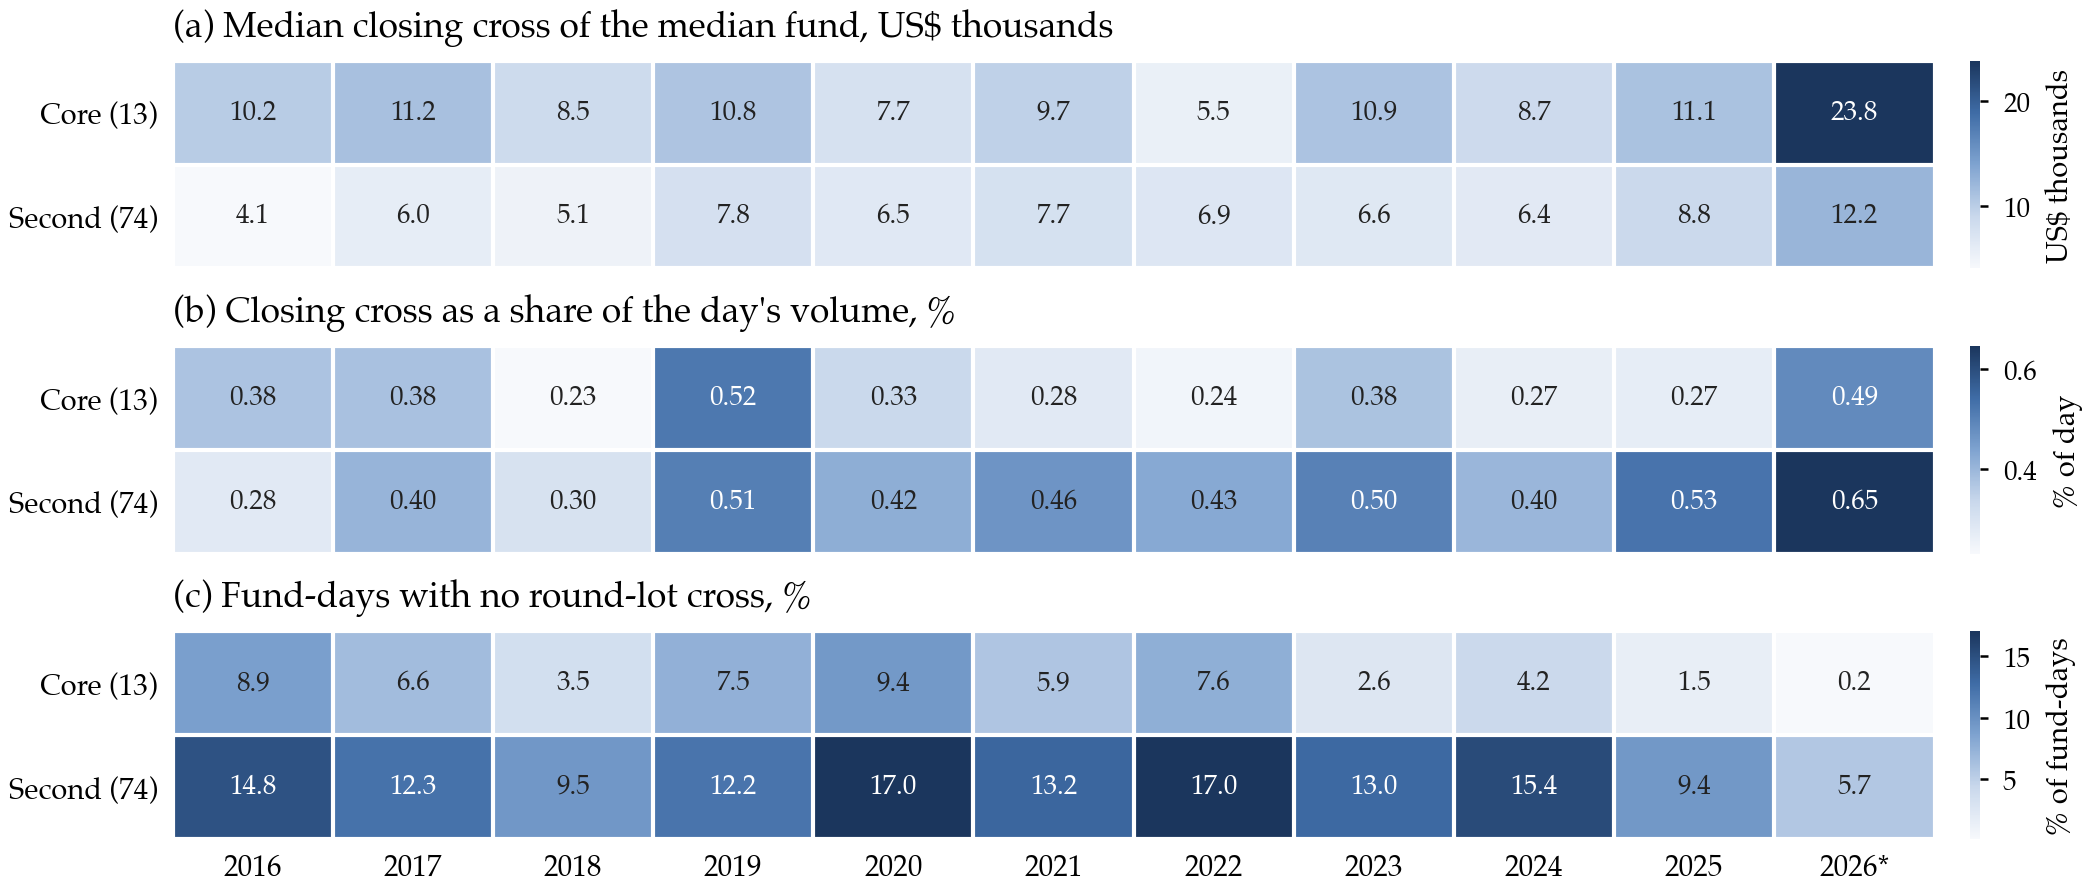
\includegraphics[width=\textwidth]{figures/fig01_cross_year_heat.png}
\caption{The closing cross by year and sleeve, 2016 to 24 November 2026 (2026$^{*}$ is year to date). (a) Median across funds of each fund's median round-lot cross, US\$ thousands. (b) The same cross as a share of the day's volume. (c) Share of fund-days with no round-lot cross (missing days excluded); before each venue's official-close data begin (late 2020 for NYSE names, 2021 for Nasdaq) a day without a cross is a label, not a reading of the tape.}
\label{fig:a_year}
\qsource{Alpaca SIP auction prints and daily bars; author's calculations.}
\end{figure*}

That level is new (Figure~\ref{fig:a_year}). The core's median fund crossed between \$5.5k and \$11.2k a year in 2016--2025, and its share of fund-days with no round-lot cross fell from 8.9\% in 2016 to 0.2\% in 2026; the second sleeve's fell from 14.8\% to 5.7\%. The rise came in steps during 2026 (Figure~\ref{fig:a_month}): the core's monthly median cross was \$14.7k--16.1k in March--May, \$25.9k in June, \$29.3k in July and \$38.0k--42.2k from August to November. The cross's share of daily volume rose with it, from 0.20--0.31\% in February--May to 0.55--0.82\% in June--August, before daily volume itself rose (to \$6.0M--7.7M a day in September--November). The second sleeve shows the same step, from about \$8k a month to \$13k--17k from June. The step began before the core paper book opened, and paper orders never reach the exchange, so the book did not cause it; its cause is not identified. A capacity figure measured on the last few months sits at the top of a decade's range and should not be read as a floor.

\begin{figure}[tbp]
\centering
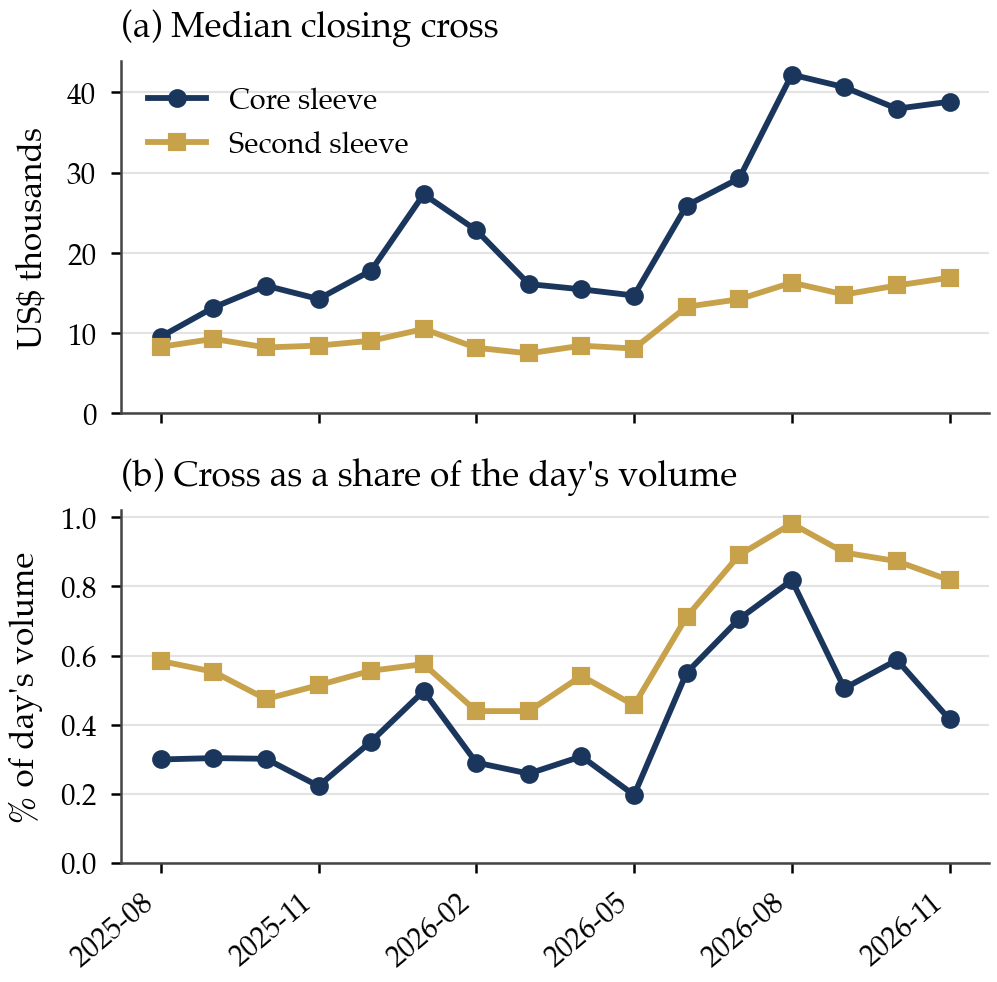
\includegraphics[width=\columnwidth]{figures/fig02_cross_monthly.png}
\caption{The 2026 step: monthly median closing cross (a) and its share of the day's volume (b), median across funds, August 2025 to November 2026.}
\label{fig:a_month}
\qsource{Alpaca SIP auction prints and daily bars; author's calculations.}
\end{figure}

\subsection{Forecasting the cross before the cut-off}

A cap on the MOC order needs a forecast of the cross made before the order is sent. The cap time is 15:45 (12:45 on a 13:00 close). The target is the log of the day's cross in dollars; a day without a cross is treated as minus infinity, so it counts against the coverage of a low quantile, as it would against a cap. A forecast for day $D$ uses only crosses and daily bars dated before $D$, five-minute bars on $D$ that end by 15:45, and calendar facts about $D$. Every rolling feature is lagged one session, and the script recomputes a sample of rows from data cut at $D$ and stops on any difference (it found none). Evaluation is out of sample, January 2017 to 24 November 2026, with the regressions refitted each month on earlier months only.

\begin{figure*}[t]
\centering
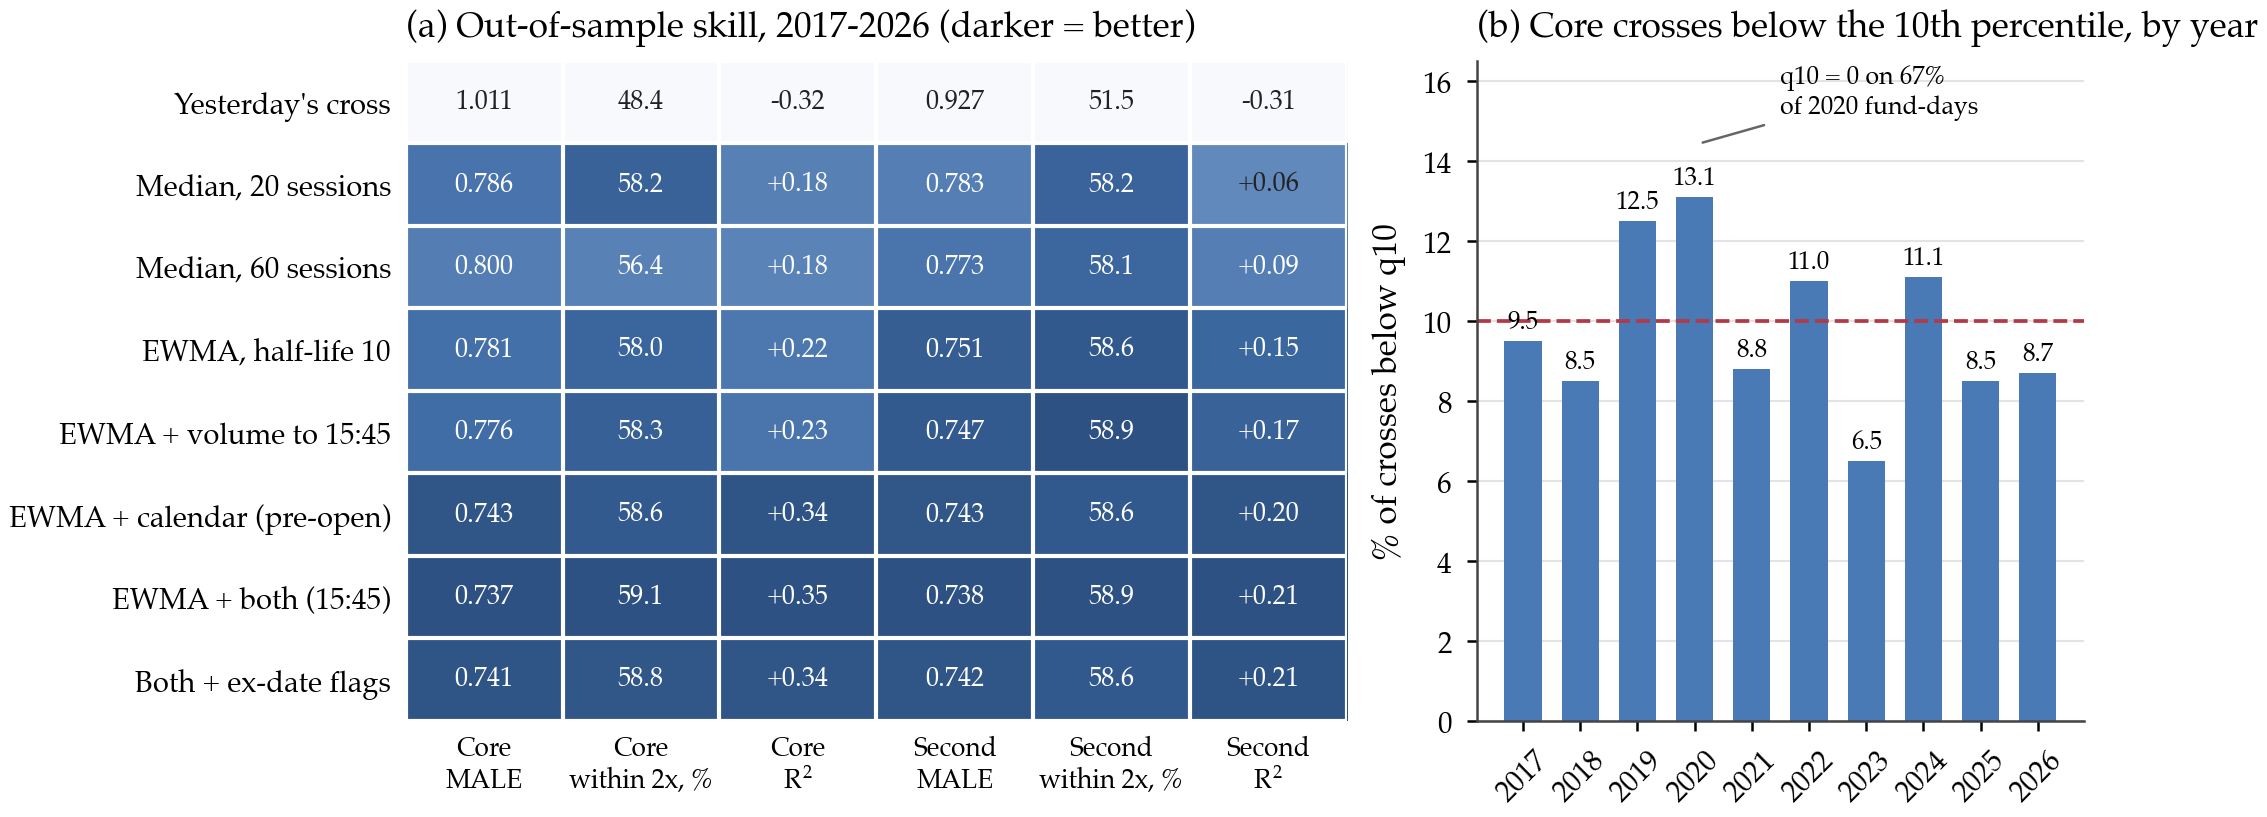
\includegraphics[width=\textwidth]{figures/fig03_forecast.png}
\caption{Forecasting the closing cross, out of sample 2017--2026. (a) Eight forecasts against six measures: MALE is the mean absolute log error; ``within 2x'' the share of name-days within a factor of 2; $R^2$ is against each fund's own full-window mean, a benchmark that uses hindsight. Shading is scaled within each column, darker for better. (b) Share of core crosses falling below the 10th-percentile forecast (q10) of the best 15:45 model, on days when q10 allows any MOC order; the dashed line marks the nominal 10\%, and in 2020 q10 was zero on 67\% of fund-days.}
\label{fig:a_fc}
\qsource{Alpaca SIP auction prints, daily and five-minute bars; author's calculations.}
\end{figure*}

Figure~\ref{fig:a_fc}(a) compares eight forecasts. The best at 15:45 combines an exponentially weighted moving average (EWMA) of the log cross with same-day volume and calendar flags; its mean absolute log error of 0.737 is a typical factor of 2.1, it is within a factor of 2 on 59\% of name-days, and its $R^2$ is 0.35 for the core and 0.21 for the second sleeve. Same-day volume helps a little: a day with twice its usual volume by 15:45 has a cross about 20\% larger, and the volume surprise correlates 0.12 with the EWMA's error. The calendar matters more (Figure~\ref{fig:a_flags}). Quarter-end crosses in the core funds are a median 25 times the fund's usual size, month-ends 2.6 times, and 13:00 closes about two-thirds; who trades at quarter-end is not identified. Ex-date flags add nothing once the calendar is in. The calendar-only model uses facts known before the open, and it is the forecast used to size the cap below.

\begin{figure}[tbp]
\centering
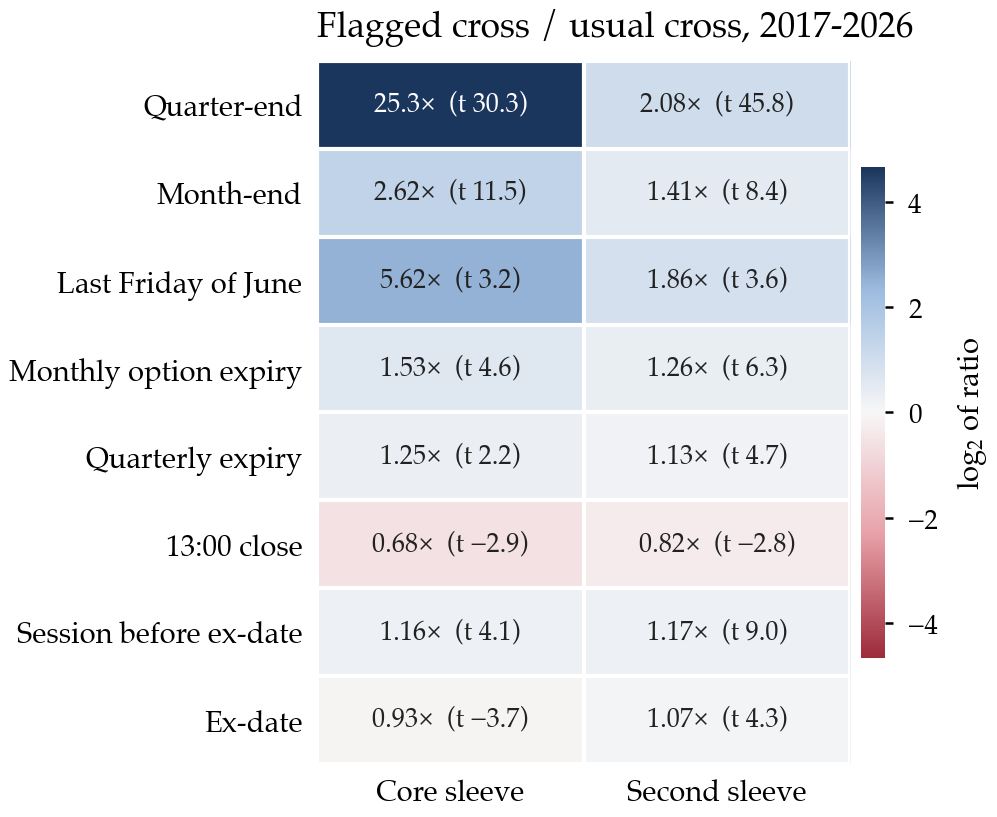
\includegraphics[width=\columnwidth]{figures/fig04_flags.png}
\caption{Calendar effects on the closing cross, round-lot days 2017--2026: median across funds of the median flagged cross over the median unflagged cross, with the $t$-statistic of the difference in mean EWMA residual, clustered by date. Shading is $\log_2$ of the ratio.}
\label{fig:a_flags}
\qsource{Alpaca SIP auction prints; author's calculations.}
\end{figure}

\textbf{Calibration.} A cap needs a low quantile, not a point forecast. The 10th and 25th percentiles (q10, q25) are the point forecast plus the empirical quantile of the pooled residuals over the previous 12 months. For the core sleeve, 9.6\% of realised crosses fell below q10 on days when q10 allowed any MOC (6.5--13.1\% by year, Figure~\ref{fig:a_fc}b) and 24.0\% fell below q25. The q10 was zero on 6.6\% of name-days, all in 2020, when days without a cross filled a tenth or more of the trailing residuals. The price of calibration is size: q10 sits at a median 0.21 of the point forecast (0.38 in the last 60 sessions). The second sleeve has so many no-cross days that its pooled q10 is zero on 79\% of name-days from 2017; quantiles taken from each fund's own last 250 days cut that to 40\%, with 9.9\% coverage on positive-cap days. The core forecast holds across eras ($R^2$ 0.20, 0.23 and 0.38 in 2016--19, 2020--22 and 2023--26), both halves (0.24 and 0.38) and both market-volatility regimes (0.39 and 0.32).

\subsection{The afternoon pool and the spread}

What does not go to the auction must be worked in the continuous market (Table~\ref{tab:a_pool}). For the median core fund, 14:00--15:50 traded \$1.83M over the last 60 sessions, 46 times the same day's cross. The time-weighted quoted half-spread for the median core fund was 4.87\,bp in every window, about one tick (3.4--11.6\,bp across funds); the second sleeve's was 15.4\,bp in 14:00--15:50, narrowing to 13.4\,bp in 15:30--15:50. Over the decade the core's median fund traded \$0.48M--0.64M a year in 14:00--15:50 through 2024 and \$1.20M in 2026. Raw SIP trades in the same windows sum to the bars' dollar volume within 0.14\% over the last five sessions.

\begin{table}[H]
\centering
\caption{Afternoon dollar volume, last 60 sessions, median fund; ``$\div$ X'' is the window over the same day's cross.}
\label{tab:a_pool}
\footnotesize
\setlength{\tabcolsep}{4pt}
\qstripes
\begin{tabular}{@{}lrrrrr@{}}
\toprule
\qhead{Window} & \qhead{\makecell[r]{Core\\US\$}} & \qhead{\makecell[r]{Core\\$\div$ X}} & \qhead{\makecell[r]{Core\\5\%}} & \qhead{\makecell[r]{Second\\US\$}} & \qhead{\makecell[r]{Second\\$\div$ X}} \\
\midrule
14:00--15:50 & 1.83M & 45.9 & 91.7k & 417k & 27.3 \\
15:00--15:50 & 0.97M & 22.5 & 48.6k & 195k & 12.4 \\
15:30--15:50 & 0.39M & 10.3 & 19.7k & 85k & 5.2 \\
\bottomrule
\end{tabular}
\qsource{Alpaca SIP five-minute bars and auction prints; author's calculations.}
\end{table}

\subsection{Does working earlier gain or lose against the close?}

For an order with side $s$ ($+1$ buy, $-1$ sell) we measure
\begin{equation}
G = s \times \frac{P_{\text{close}} - P_{\text{ref}}}{P_{\text{ref}}}\ \text{(bp)},
\end{equation}
so $G>0$ means the close was worse for our side than the reference price, and working at the reference would have gained before spread and impact. Means are weighted by notional and $t$-statistics are computed across days. These are the book's own orders, so the results are conditional on the signal's direction.

\begin{figure*}[t]
\centering
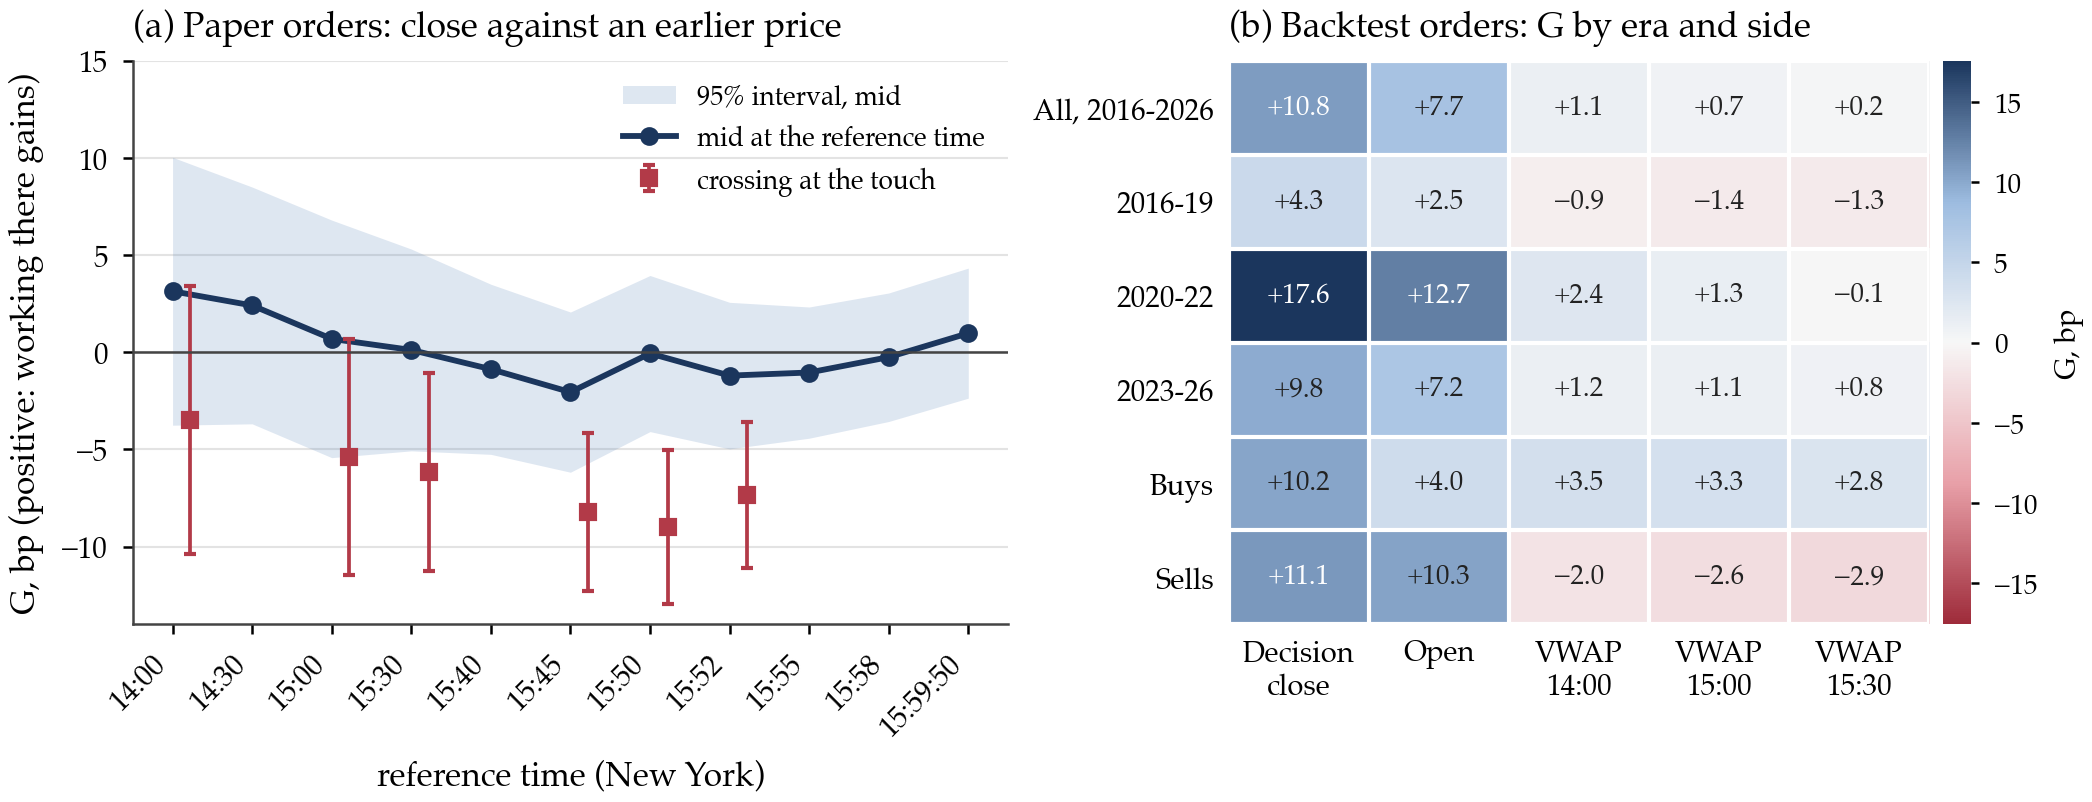
\includegraphics[width=\textwidth]{figures/fig05_path.png}
\caption{The price path into the close, in the book's trade direction. (a) Core paper orders sent shortly before the close, 2026-09-30 to 11-24 (263 orders, 35 sessions): day-mean $G$ against the mid at each reference time with its 95\% interval, and against crossing the spread at the touch. (b) The policy's backtest orders, 2016--2026 (6,331 orders, 1,470 days): day-mean $G$ against five references by era and side.}
\label{fig:a_path}
\qsource{Alpaca SIP quotes, bars and auction prints; Alpaca paper-account orders; author's calculations.}
\end{figure*}

Figure~\ref{fig:a_path} gives three results. First, from 14:00 the path to the close is flat for these orders: +1.11\,bp against the 14:00--15:50 VWAP over the decade ($t$ 1.97; $-$0.89, +2.38 and +1.23\,bp by era) and +0.27\,bp on paper ($t$ 0.10). Second, the split by side shows the small average is not a signal effect: buys gain +3.54\,bp and sells lose $-$2.02\,bp against the 14:00--15:50 VWAP, so these funds' prices rise into the close on average whichever way the book trades. Third, the move in the book's favour happens earlier, between the decision-day close and the early afternoon (+10.8\,bp over the decade, +20.7\,bp on paper). Crossing the spread costs about the half-spread ($-$7.3 to $-$9.0\,bp at the touch on paper between 15:45 and 15:52).

\subsection{A cap rule and capacity}
\label{sec:a_cap}

The rule measured is
\begin{equation}
\text{MOC}_i = \min\left(\text{order}_i,\ c \times \widehat{q}_{10,i}\right),
\end{equation}
with the rest worked in the afternoon. The split must be fixed before the working window opens, so it is sized from the pre-open forecast. Orders are scaled linearly with book size from the core paper account's orders in steady state (2026-10-01 to 11-24: 256 orders, 34 sessions). The cross and the pool are each day's own, measured without the book in them.

\begin{table*}[t]
\centering
\caption{Capacity at four book sizes, core paper orders scaled linearly, 2026-10-01 to 11-24. ``Order $\div$ cross'' is the notional-weighted median of each order over the day's cross; the cap is $c$ times the pre-open 10th-percentile forecast; the remainder is the worked-weighted median of worked notional over the day's 14:00--15:50 dollar volume at $c$ = 33\%.}
\label{tab:a_cap}
\footnotesize
\qstripes
\begin{tabular}{@{}lrrrrrrrr@{}}
\toprule
\qhead{Book} & \qhead{\makecell[r]{Median\\order}} & \qhead{\makecell[r]{90th pct\\order}} & \qhead{\makecell[r]{Order\\$\div$ cross}} & \qhead{\makecell[r]{Notional\\above cross}} & \qhead{\makecell[r]{MOC share\\$c$ = 10\%}} & \qhead{\makecell[r]{MOC share\\$c$ = 20\%}} & \qhead{\makecell[r]{MOC share\\$c$ = 33\%}} & \qhead{\makecell[r]{Remainder\\$\div$ pool}} \\
\midrule
\$100k & \$2.7k & \$12.8k & 21.6\% & 8.0\% & 27.3\% & 43.2\% & 57.2\% & 0.6\% \\
\$1M & \$26.6k & \$128k & 216\% & 74\% & 4.0\% & 7.5\% & 11.4\% & 5.7\% \\
\$5M & \$133k & \$638k & 1,082\% & 96\% & 0.8\% & 1.6\% & 2.7\% & 25.5\% \\
\$10M & \$266k & \$1.28M & 2,164\% & 99\% & 0.4\% & 0.8\% & 1.4\% & 51.2\% \\
\bottomrule
\end{tabular}
\qsource{Alpaca paper-account orders; Alpaca SIP auction prints and five-minute bars; author's calculations.}
\end{table*}

\begin{figure*}[t]
\centering
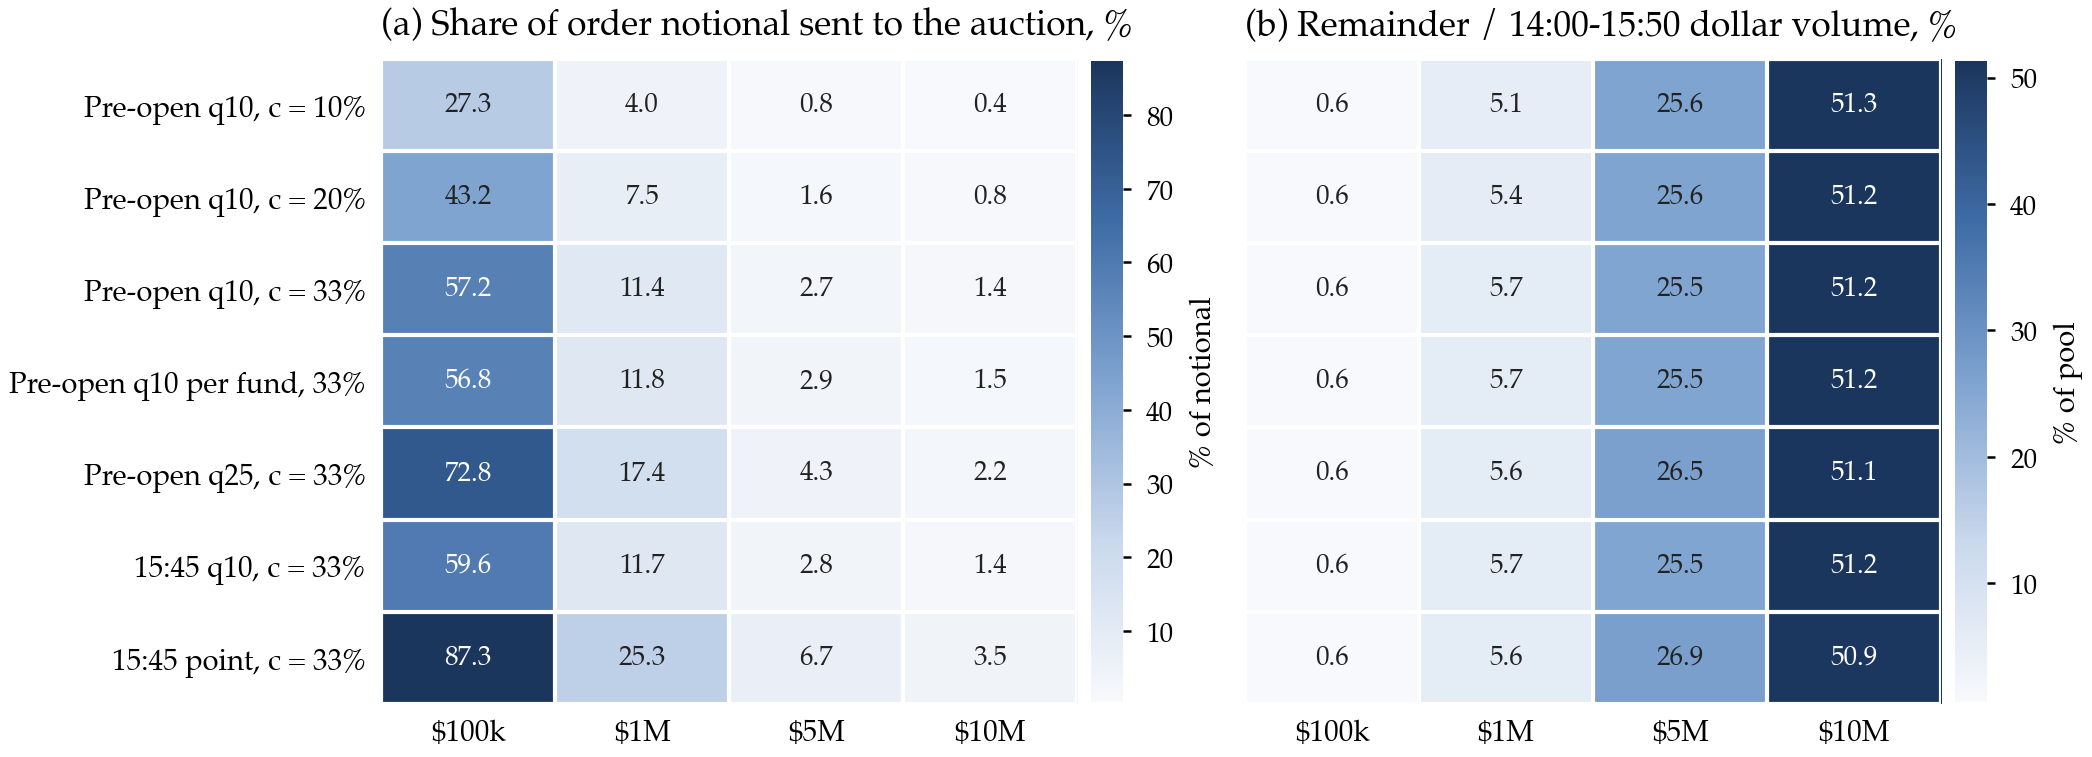
\includegraphics[width=\textwidth]{figures/fig06_capacity.png}
\caption{Capacity by cap rule and book size, core paper orders scaled linearly, 2026-10-01 to 11-24. (a) Share of order notional that the cap sends to the closing auction. (b) The remainder as a share of the same day's 14:00--15:50 dollar volume (worked-weighted median). Rules use the pre-open forecast (pooled or per-fund quantiles) or the 15:45 forecast.}
\label{fig:a_cap}
\qsource{Alpaca paper-account orders; Alpaca SIP auction prints and five-minute bars; author's calculations.}
\end{figure*}

Table~\ref{tab:a_cap} and Figure~\ref{fig:a_cap} give the answer. At about \$100k, a cap of a third of q10 keeps 57\% of the notional in the auction and the rest is 0.6\% of the 14:00--15:50 pool: the close and the afternoon together are ample. At \$1M only 4--11\% can go to the auction and the rest is 5.7\% of the pool, with 27.5\% of the worked notional above a tenth of it. At \$5M and \$10M the afternoon binds too: the remainder is a quarter and a half of the 14:00--15:50 pool, and the book would need the whole session, more than one day for its largest trades, or a slower trading rule. This is a statement about the size of the book's trades against the market, not a cost estimate. Under the cap the MOC order is a median 3--14\% of the realised cross and exceeds $c$ on 4--13\% of orders. The choice of forecast barely matters: the 15:45 forecast moves the \$100k MOC share from 57.2\% to 59.6\%, and only a cap on the point forecast, which is breached far more often, sends much more. The policy's backtest orders since 2023 give a similar picture (MOC share 35\%, 6.4\%, 1.5\% and 0.8\% at the four sizes). Per fund and day, a third of the pre-open q10 allows a median \$4,576 of MOC in a core fund (\$2,310--21,029 across funds) and \$1,446 in a second-sleeve fund (\$149--7,495).

\subsection{What cannot be measured without real money}

Paper cannot give our impact on the closing print, whether offsetting interest arrives when our order joins the auction, or the impact of a worked order (paper does not check order quantity against the displayed quote). Every participation figure above is our size against a cross that did not contain us.

The smallest real-money measurement is to run the core book live with MOC orders at about its paper size, where its orders are already a notional-weighted median of 22\% of the cross, and to score each order's signed print-minus-mid against the paper record. On the last 100 sessions the closing print sits a standard deviation of 17.0\,bp from the 15:59:50 mid. Signed by our side, the paper orders' print-minus-mid is +0.98\,bp a day ($t$ 0.58, daily s.d.\ 10.1\,bp, 35 sessions): the impact-free baseline. Table~\ref{tab:a_power} gives the live sessions needed.

\begin{table}[H]
\centering
\caption{Live MOC sessions needed to detect an impact on the closing print (80\% power, 5\% two-sided, 15:59:50 mid basis).}
\label{tab:a_power}
\footnotesize
\qstripes
\begin{tabular}{@{}rrr@{}}
\toprule
\qhead{Impact} & \qhead{vs 35-session paper record} & \qhead{vs unlimited record} \\
\midrule
10\,bp & 11 & 8 \\
5\,bp & 368 & 32 \\
2\,bp & not reachable & 200 \\
\bottomrule
\end{tabular}
\qsource{Alpaca SIP quotes and auction prints; Alpaca paper-account orders; author's calculations.}
\end{table}

The paper record is the binding constraint for small impacts; it grows by a session a day. Historical imbalance data would show how much closing interest stands on each side without us, but no free source carries it. Alpaca has no imbalance history, and its real-time imbalance message carries no quantity \cite{alpacarealtime}. NYSE's proprietary imbalance feed publishes paired and imbalance quantities every second during the auction for every traded name \cite{nyseimbalance}; its history is sold at \$1,000 a month with a 12-month minimum, plus \$500 a month for NYSE American \cite{nysepricing}. It would still not measure our own impact.

%═══════════════════════════════════════════════════════
\section{Study 2: Market Beta of the Second Sleeve}
\label{sec:beta}

\subsection{Question and design}

The second sleeve holds 74 funds in five families. Over its first 13 paper sessions its daily return moved against the market: the same-day beta of the paper account's return to SPY was $-$0.44. We ask whether the sleeve's market tilt can be removed without hurting it, and which of two approaches is better: reweight the funds themselves to zero beta, or leave the book unchanged and hold an SPY position against its beta.

The base is the sleeve as the paper account trades it, rebuilt from the same construction and scored on the desk's research harness with the decide-$t$, fill-$t{+}1$, earn-$t{+}2$ convention. Returns are CRSP daily total returns (via WRDS) to 31 December 2024 and, after that, total returns built from daily prices and distribution records. From 2005 to 2022 the base reproduces an independently implemented series of the same book to $6\times10^{-17}$ over 4,497 sessions; for 2023--2026 there is no independent check, and the base matches an earlier result from the same code, which confirms the plumbing but not the construction.

Each variant (Table~\ref{tab:b_var}) starts from the base's target on every day, changes one thing, is rescaled to the base's ex-ante volatility, and then goes through the same no-trade band and limits. The projected variants take the least-squares closest target with zero exposure to the stated columns.

\begin{table}[H]
\centering
\caption{The variants. The code name is the label in Figure~\ref{fig:b_eq}.}
\label{tab:b_var}
\footnotesize
\qstripes
\begin{tabularx}{\columnwidth}{@{}l>{\raggedright\arraybackslash}X@{}}
\toprule
\qhead{Code name} & \qhead{What changes} \\
\midrule
\texttt{base} & nothing: the sleeve as traded \\
\texttt{beta\_spy} & zero dollar and zero SPY beta \\
\texttt{beta\_cef} & zero dollar and zero beta to the equal-weight return of the 74 funds \\
\texttt{family} & dollar-neutral within each family \\
\texttt{family\_beta} & family-neutral and zero SPY beta \\
placebo (8 seeds) & zero exposure to a fake ``beta'': each day's sorted betas assigned to the funds in a fixed random order, so it has beta's spread and persistence and nothing else \\
\texttt{spy\_hedge} & base book plus SPY at minus the book's ex-ante beta \\
short-only & the same SPY position, only on days the ex-ante beta is negative \\
\bottomrule
\end{tabularx}
\qsource{Study design.}
\end{table}

\textbf{Betas.} Each fund's beta is the Dimson \cite{dimson1979} sum of slopes on SPY at lags 0, 1 and 2, estimated by ordinary least squares on the 252 sessions strictly before the decision date; the script asserts this on both the date labels and the data rows. A one-factor model is used because the credit and preferred-stock ETFs start in 2007 and the sleeve in 2005; against the four-factor exposure model used elsewhere on the desk, the equity loading correlates 0.87--0.99 per fund. Two regime splits were named before any regime row was read: VIX at or above its trailing 252-session median against below it, and SPY's trailing 126-session return negative against not. The tilt-state rows use the base's ex-ante beta at $\pm$0.2, a threshold chosen after reading the beta distribution but before any return in those states was computed.

\subsection{Results}

\begin{table*}[t]
\centering
\caption{The second sleeve and its variants, 2005-02-22 to 2026-09-30, gross. NW $t$: Newey--West \cite{newey1987} $t$ of the mean. Realised beta: daily regression on SPY. Held ex-ante beta: mean (mean absolute) of the held book. $\Delta$Sharpe $p$: Ledoit--Wolf \cite{ledoit2008} test against the base, block bootstrap (block 42, 1,999 draws). Placebo: mean over eight seeds, range in the next row.}
\label{tab:b_head}
\footnotesize
\setlength{\tabcolsep}{4.2pt}
\qstripes
\begin{tabular}{@{}lrrrrrrrrr@{}}
\toprule
\qhead{Variant} & \qhead{Ann.\ \%} & \qhead{Vol \%} & \qhead{Sharpe} & \qhead{NW $t$} & \qhead{Max DD \%} & \qhead{Turn/yr} & \qhead{Realised $\beta$ ($t$)} & \qhead{Held ex-ante $\beta$} & \qhead{$\Delta$Sharpe ($p$)} \\
\midrule
Base & 11.41 & 7.23 & 1.58 & 7.9 & $-$7.5 & 52.2 & +0.047 (+2.7) & +0.061 (0.166) & --- \\
SPY-beta-neutral & 10.99 & 7.36 & 1.49 & 7.4 & $-$20.7 & 62.8 & $-$0.066 ($-$3.4) & $-$0.027 (0.097) & $-$0.09 (0.51) \\
CEF-beta-neutral & 11.01 & 7.41 & 1.49 & 7.3 & $-$18.6 & 63.3 & $-$0.075 ($-$3.8) & $-$0.044 (0.117) & $-$0.09 (0.46) \\
Family-neutral & 12.00 & 7.51 & 1.60 & 7.9 & $-$11.4 & 54.3 & +0.032 (+1.4) & +0.089 (0.177) & +0.02 (0.84) \\
Family + SPY-beta & 12.00 & 7.21 & 1.66 & 8.1 & $-$16.2 & 69.6 & $-$0.049 ($-$3.2) & $-$0.007 (0.083) & +0.08 (0.58) \\
Placebo, mean & 10.69 & 7.31 & 1.46 & 7.3 & $-$9.1 & 56.5 & +0.029 & +0.049 (0.167) & --- \\
\quad range, 8 seeds & 9.05--11.98 & & 1.23--1.62 & & $-$7.0 to $-$12.5 & & $-$0.02 to +0.07 & & \\
\textbf{SPY overlay} & 10.28 & 7.15 & 1.44 & 7.2 & $-$9.1 & 64.3 & $-$0.001 ($-$0.1) & 0.000 (0.000) & $-$0.14 (0.08) \\
Short-only overlay & 12.07 & 7.35 & 1.64 & 8.3 & $-$8.5 & 56.4 & +0.090 (+5.2) & +0.113 (0.113) & +0.06 (0.17) \\
\bottomrule
\end{tabular}
\qsource{CRSP via WRDS; fund prices and distributions after 2024; Yahoo Finance (SPY); author's calculations.}
\end{table*}

\begin{figure*}[t]
\centering
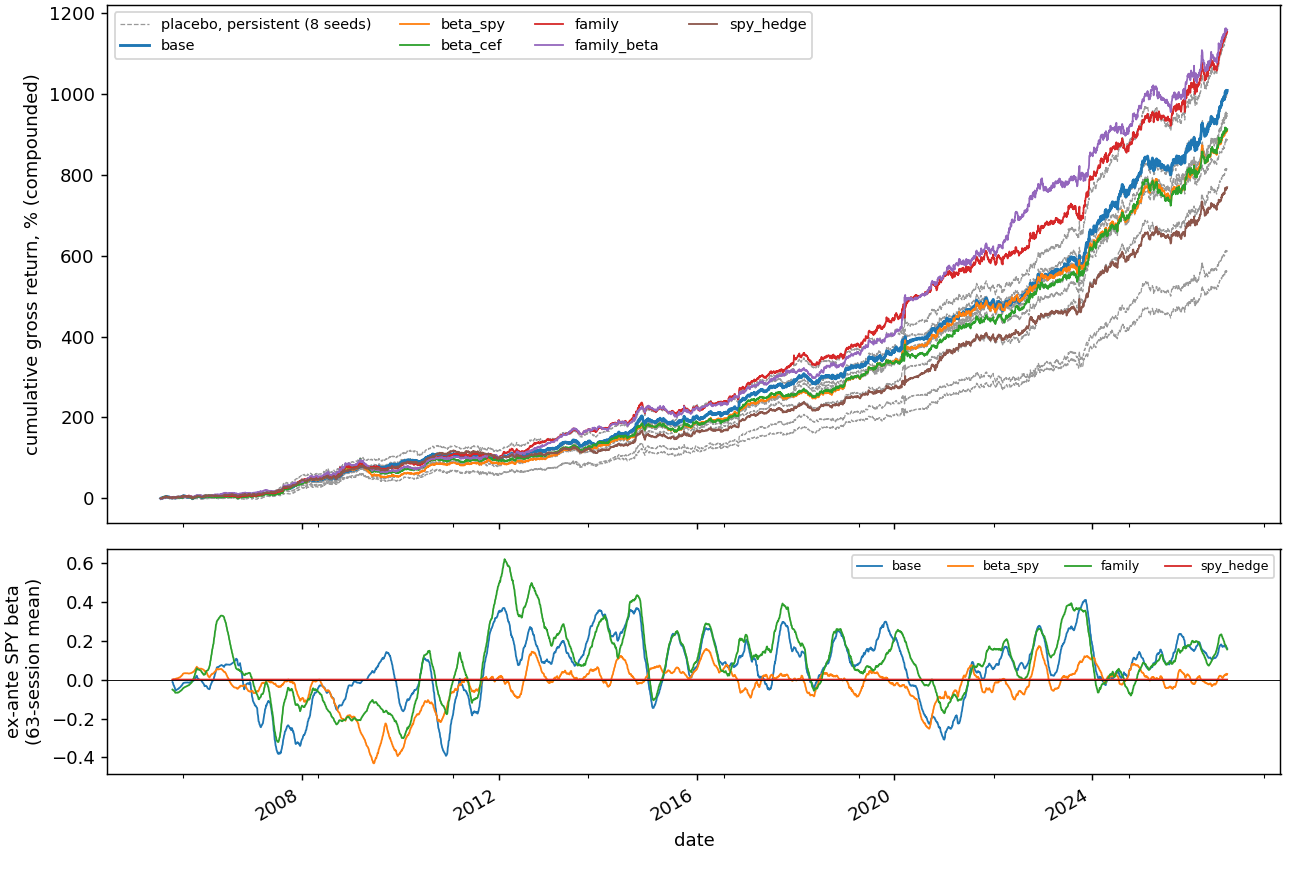
\includegraphics[width=0.66\textwidth]{figures/fig07_beta_equity.png}
\caption{The second sleeve and its variants, gross, 2005--2026, reproduced from the study's output (its daily series are not among the published aggregates). Top: cumulative compounded gross return, \%; the grey dashed lines are the eight placebo seeds. Bottom: ex-ante SPY beta of the decided book, 63-session mean. Code names are defined in Table~\ref{tab:b_var}.}
\label{fig:b_eq}
\qsource{CRSP via WRDS; fund prices and distributions after 2024; Yahoo Finance (SPY); author's calculations.}
\end{figure*}

Table~\ref{tab:b_head} and Figures~\ref{fig:b_eq} and \ref{fig:b_dots} give the headline. The base earned 11.4\% a year gross at 7.2\% volatility, a Sharpe ratio of 1.58, with a small positive realised beta (+0.047).

\textbf{Reweighting does not help.} Projecting the target onto zero SPY beta gives a Sharpe of 1.49. That loss is not evidence about beta: the placebo, which removes a fake direction with the same spread and persistence as beta, scores 1.23 to 1.62 over eight seeds, so removing any persistent direction from this book costs about that much. What is specific to beta lies outside the placebo's range, and it goes against reweighting. The SPY-beta-neutral book's maximum drawdown is $-$20.7\%, in the rebound of March to August 2009, against the placebo's $-$7.0\% to $-$12.5\% and the base's $-$7.5\%. Its 2023--2026 Sharpe is 1.73, against the placebo's 1.79--2.18 and the base's 2.06, and its realised beta overshoots to $-$0.066. One reading, consistent with these rows but not measured fund by fund, is that after a sell-off the cheap funds are the high-beta ones, and trailing crash-period betas told the projection to short them into the rebound. Neutralising within families alone leaves the beta in place.

\begin{figure*}[t]
\centering
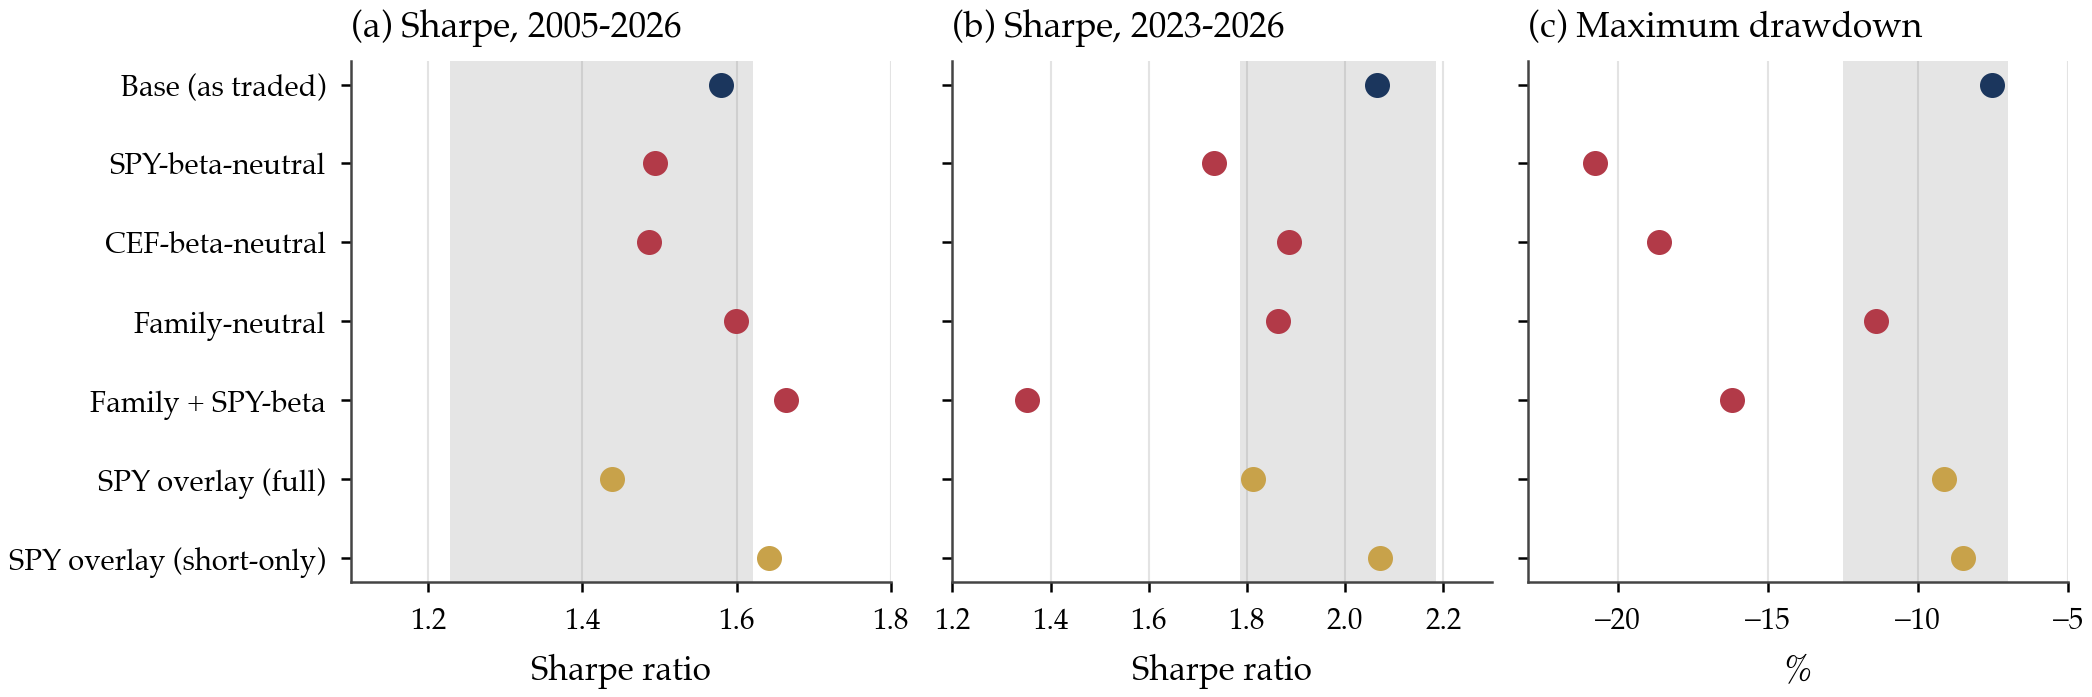
\includegraphics[width=\textwidth]{figures/fig08_variants.png}
\caption{The variants against a placebo, 2005-02-22 to 2026-09-30, gross. Each dot is one variant's full-sample Sharpe ratio (a), 2023--2026 Sharpe ratio (b) and maximum compounded drawdown (c); the grey band is the range of eight placebo seeds. Navy: the base; gold: the two SPY overlays; red: the reweighted books.}
\label{fig:b_dots}
\qsource{CRSP via WRDS; fund prices and distributions after 2024; Yahoo Finance (SPY); author's calculations.}
\end{figure*}

\textbf{An overlay removes the beta.} Holding SPY at minus the book's ex-ante beta brings the realised beta to $-$0.001 with almost no change in volatility (7.15\% against 7.23\%). The cost is weak evidence of about 1.1\% a year (10.28\% against 11.41\%, $\Delta$Sharpe $-$0.14, $p$ 0.08). Neighbouring choices form a plateau: with beta windows of 63, 126 and 504 sessions the overlay's Sharpe is 1.45, 1.45 and 1.44, and 1.51 with a same-day-only beta; a hedge only beyond $\pm$0.1, $\pm$0.2 or $\pm$0.3 of beta scores 1.53, 1.56 and 1.60.

\subsection{Splits, regimes and tilt states}

\begin{figure}[tbp]
\centering
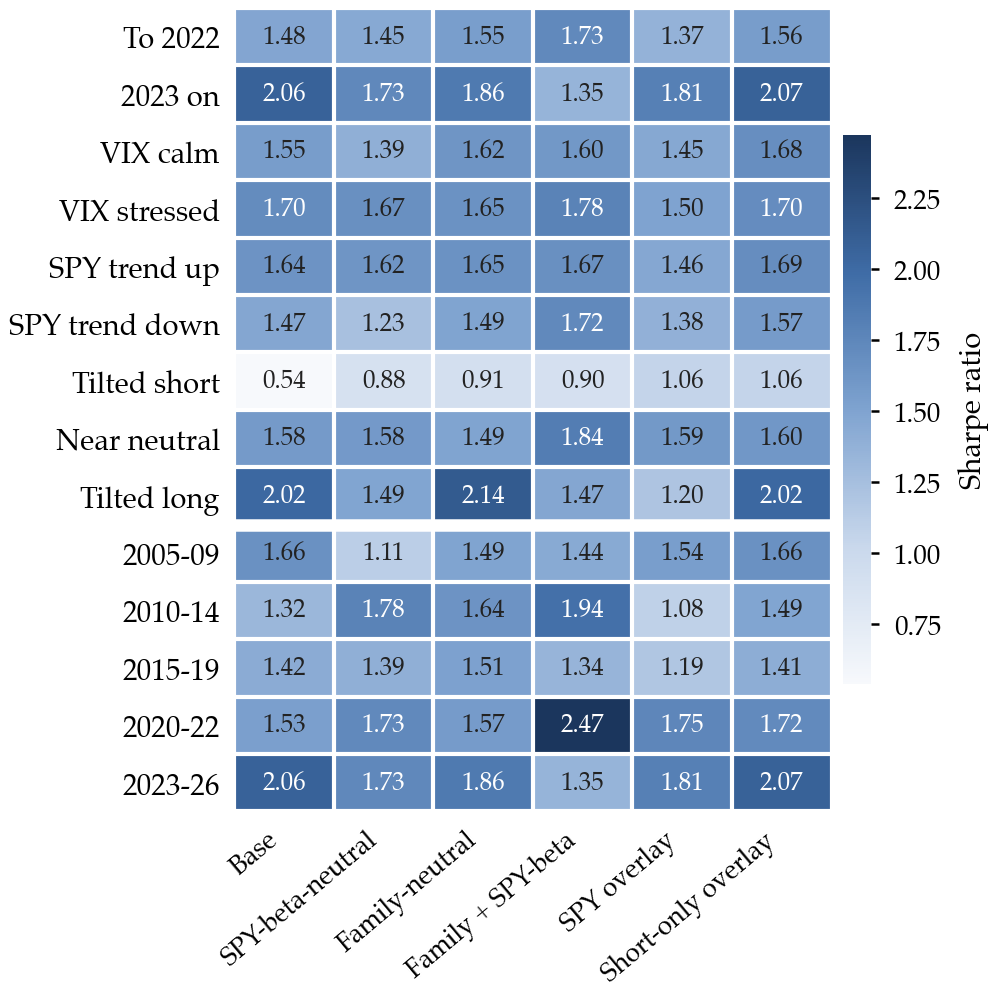
\includegraphics[width=\columnwidth]{figures/fig09_split_heat.png}
\caption{Sharpe ratio of each variant by time split, regime, base tilt state (top block) and era (bottom block), 2005--2026, gross. Tilt states use the base's ex-ante beta at $\pm$0.2.}
\label{fig:b_split}
\qsource{CRSP via WRDS; fund prices and distributions after 2024; Yahoo Finance (SPY, VIX); author's calculations.}
\end{figure}

Every variant holds in both halves of the sample and in both regimes of each split (Figure~\ref{fig:b_split}); none beats the base after 2022, and the short-only overlay ties it. The years before 2013 hold few funds and are thin.

\textbf{The overlay over-hedges short states and pays for long ones.} When the base is tilted short its ex-ante beta averages $-$0.32 while its realised beta is only $-$0.10, so the full hedge turns that state's realised beta to +0.21, though it lifts the state's return from 3.9\% to 8.5\% a year. When the base is tilted long, its beta was paid: 15.0\% a year, which the hedge takes to 8.2\%. Almost all of the overlay's cost falls on those long-tilt days.

\textbf{The short-only overlay is mostly a constant long SPY position.} It holds SPY on 35\% of days with a mean weight of +0.053, and its realised beta is +0.09 ($t$ 5.2). The base plus a constant 0.053 of SPY every day scores 1.625, against the short-only overlay's 1.642 and the base's 1.580. Shifting the short-only weight series in time by a random offset of at least a year keeps its level and persistence and destroys its timing; 14\% of 500 such shifts score at least as well. Its small gain is an average long equity position, not a hedge that knows when to act.

\textbf{Tilt states.} Over 2005--2026 the base's ex-ante beta has a 5th--95th percentile range of $-$0.31 to +0.37 and a mean of +0.06. On the 563 sessions when it was at or below $-$0.2 (180 of them in 2007, 76 in 2010 and 146 in 2020--21; none from January to September 2026) the sleeve earned 3.9\% a year against 12.3\% on the rest. The difference, $-$8.4\% a year, has a standard error of 5.1 clustered by episode ($t$ $-$1.64, 86 episodes); clustering by 21-session blocks gives $t$ $-$1.65, and an episode bootstrap of the short state's Sharpe of 0.54 gives a 90\% range of $-$0.56 to 1.75. That is weak evidence and not a forecast for the live sleeve, whose ex-ante beta is currently in that state.

\subsection{The paper window}

We applied the overlay to the paper account's official end-of-day return over its 13 trading sessions (2026-11-05 to 11-23). The SPY weight is decided on each evening's plan as minus that plan's ex-ante SPY beta and earns the session two days later, as in the backtest. The weights were 0.26 to 0.33 of capital long SPY; every plan's beta was negative, so the short-only form is identical here.

\begin{figure}[tbp]
\centering
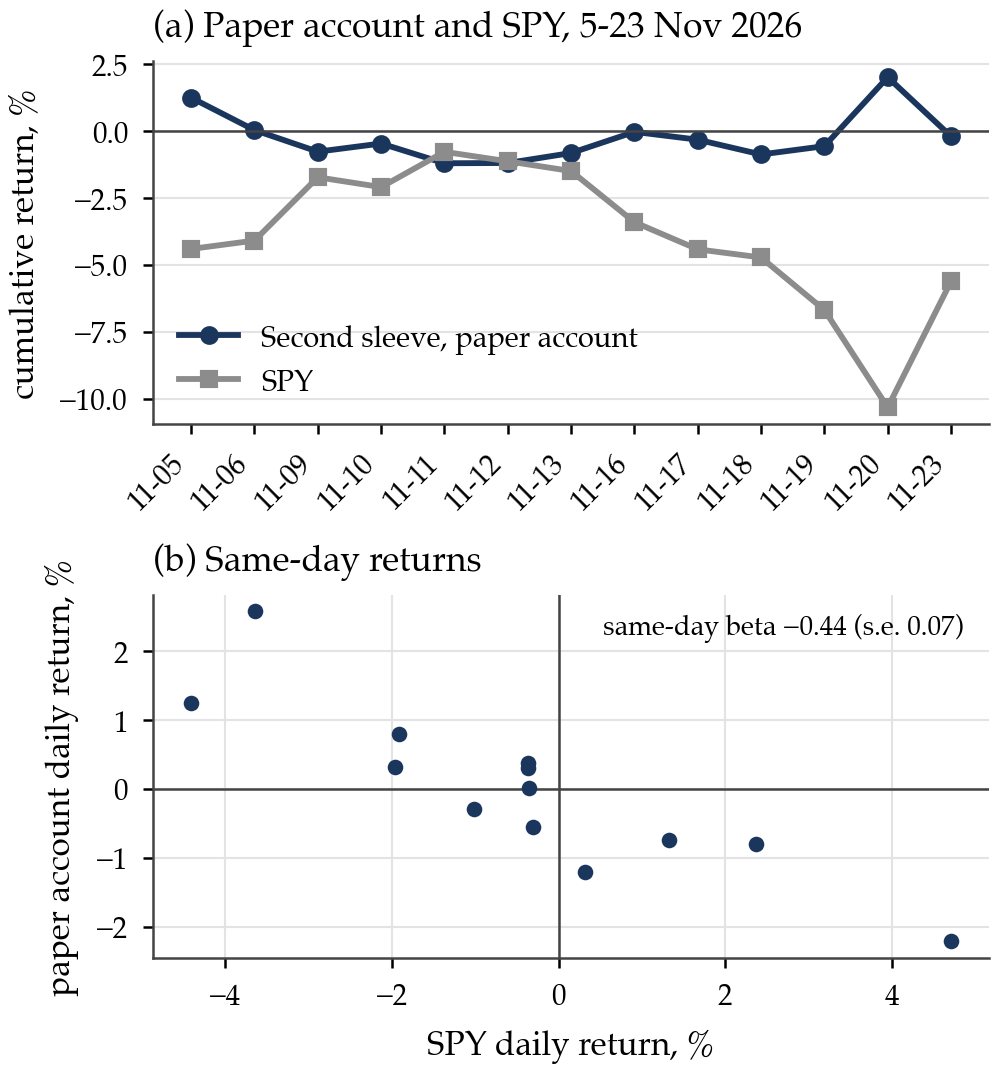
\includegraphics[width=\columnwidth]{figures/fig10_live.png}
\caption{The second sleeve's paper account over its first 13 sessions, 2026-11-05 to 11-23. (a) Cumulative sum of daily returns of the paper account and of SPY. (b) Daily paper-account return against SPY's, with the same-day OLS beta. Paper-account results, not live trading.}
\label{fig:b_live}
\qsource{Alpaca paper-account end-of-day equity; Yahoo Finance (SPY); author's calculations.}
\end{figure}

\begin{table}[H]
\centering
\caption{Paper-account return of the second sleeve, 2026-11-05 to 11-23 (13 sessions), with and without the SPY overlay. Paper-account results, not live trading.}
\label{tab:b_live}
\footnotesize
\qstripes
\begin{tabular}{@{}lrr@{}}
\toprule
 & \qhead{Paper account} & \qhead{+ SPY overlay} \\
\midrule
Sum of daily returns & $-$0.20\% & $-$2.09\% \\
Annualised volatility & 18.94\% & 10.19\% \\
Same-day SPY beta (s.e.) & $-$0.443 (0.068) & $-$0.151 (0.067) \\
Worst day & $-$2.21\% & $-$1.12\% \\
Best day & +2.58\% & +1.44\% \\
Vol.\ without 3 largest SPY days & 10.15\% & 6.97\% \\
\bottomrule
\end{tabular}
\qsource{Alpaca paper-account end-of-day equity; Yahoo Finance (SPY); author's calculations.}
\end{table}

Figure~\ref{fig:b_live} and Table~\ref{tab:b_live} show that the overlay would have cut volatility nearly in half and the same-day beta from $-$0.44 to $-$0.15, and that it would have cost 1.89\% of capital: the SPY leg was long about 0.30 of capital while SPY fell 5.6\% (sum of daily returns). SPY ran at 38\% annualised volatility in this window, and three days carry most of the variance. The betas compared are of two kinds: the $-$0.44 and $-$0.15 are same-day betas on 13 points, while the hedge was sized on a trailing Dimson beta of $-$0.26 to $-$0.33. The realised beta exceeded the trailing estimate, so the hedged return kept a residual tilt. A simulation of every variant over the same window, rebuilt from the live price panel, follows the paper record in direction (daily correlation 0.95 for the base) but runs at 0.64--1.37 times the account's gross; in it the reweighted variants did not remove the tilt (SPY-beta-neutral kept $-$0.31). Thirteen sessions say little about return.

\subsection{Exposures and capacity}

Table~\ref{tab:b_exp} reports exposures to four factors (equity, term, credit and preferreds, proxied by SPY, IEF, HYG and PFF and orthogonalised in that order) over 2007--2026, with Dimson lags 0--2 and HAC standard errors. The overlay's equity loading is +0.004 ($t$ 0.3); every variant keeps an alpha of 10.6--12.7\% a year with $t$ between 6.7 and 7.8, and the correlation with the core sleeve's backtest is 0.02--0.06.

\begin{table}[tbp]
\centering
\caption{Factor betas and alpha, 2007-04-16 to 2026-09-30 ($t$ in brackets), and full-sample correlation with the core sleeve.}
\label{tab:b_exp}
\footnotesize
\setlength{\tabcolsep}{3pt}
\qstripes
\begin{tabular}{@{}lrrrrr@{}}
\toprule
\qhead{Variant} & \qhead{Equity} & \qhead{Credit} & \qhead{Pref.} & \qhead{$\alpha$ \%/yr} & \qhead{$\rho$ core} \\
\midrule
Base & +0.054 (3.3) & $-$0.028 & $-$0.046 & 11.2 (6.9) & 0.05 \\
SPY-$\beta$-neutral & $-$0.050 ($-$3.0) & $-$0.083 & $-$0.101 & 11.8 (7.2) & 0.02 \\
Family-neutral & +0.043 (2.1) & $-$0.055 & $-$0.088 & 11.8 (6.8) & 0.06 \\
Family + $\beta$ & $-$0.037 ($-$2.5) & $-$0.074 & $-$0.076 & 12.7 (7.8) & 0.03 \\
SPY overlay & +0.004 (0.3) & $-$0.068 & $-$0.023 & 10.6 (6.7) & 0.04 \\
Short-only & +0.099 (6.2) & $-$0.053 & $-$0.051 & 11.3 (7.0) & 0.05 \\
\bottomrule
\end{tabular}
\qsource{CRSP via WRDS; Yahoo Finance (SPY, IEF, HYG, PFF); author's calculations.}
\end{table}

Capacity (Table~\ref{tab:b_cap}) is measured on the base over 2023--2026, as every variant holds nearly the same funds. At \$1M the largest position is 17\% of a fund's 63-day average daily volume (ADV); at \$5M a third of held fund-days exceed 5\% of ADV. The backtest's largest single-fund position reached 0.69 of capital in 2023, and that concentration, not the hedge, is what limits the sleeve above \$1M. The overlay adds one SPY position, at most 0.73 of capital in the backtest; SPY's own ADV was not measured in this run.

\begin{table}[H]
\centering
\caption{Second-sleeve capacity, 2023-01-03 to 2026-09-30: positions and trades against each fund's 63-session ADV through $t-1$.}
\label{tab:b_cap}
\footnotesize
\setlength{\tabcolsep}{4pt}
\qstripes
\begin{tabular}{@{}lrrrrr@{}}
\toprule
\qhead{Capital} & \qhead{\makecell[r]{Max\\position}} & \qhead{\makecell[r]{99th\\pct}} & \qhead{\makecell[r]{Days\\$>$5\%}} & \qhead{\makecell[r]{Days\\$>$10\%}} & \qhead{\makecell[r]{Max\\trade}} \\
\midrule
\$1M & 17.0\% & 7.9\% & 3.7\% & 0.3\% & 15.1\% \\
\$5M & 85.1\% & 39.6\% & 34.8\% & 19.5\% & 75.7\% \\
\$10M & 170.1\% & 79.2\% & 44.8\% & 34.8\% & 151.3\% \\
\bottomrule
\end{tabular}
\qsource{CRSP via WRDS; fund prices after 2024; author's calculations.}
\end{table}

\subsection{Conclusion of the study}

The reweighted books are set aside: their Sharpe loss is what removing any persistent direction costs, and what is specific to beta (the 2009 drawdown, the late-period loss and an over-corrected beta) goes against them. They would be worth reopening with shrunk betas \cite{vasicek1973}, with neutrality imposed on the held book after the trading band rather than on the target, or with a band derived for this sleeve. The full SPY overlay is kept for further testing as a simulated book beside the paper sleeve. It is a separate position that leaves the sleeve's signal and holdings alone, it removed the beta in the backtest and most of it on the paper record, and its costs are measured. It will lose money whenever the market rises against a short-tilted book and gain when it falls; that is what removing the tilt means. The short-only overlay is not recommended on its own evidence; if it is run, a constant SPY position at its mean weight must run beside it as a control.

%═══════════════════════════════════════════════════════
\section{Study 3: A Leveraged-ETF Close Test}
\label{sec:etf}

\subsection{Mechanism}

A daily-reset fund with multiple $L$ must end each day with exposure $L$ times its assets $A$. After the underlying moves $r$ from the prior close, the fund holds $LA(1+r)$ of exposure against a target of $LA(1+Lr)$, so it must trade
\begin{equation}
\Delta = L(L-1)\,A\,r
\end{equation}
in the underlying, in the direction of the move, whatever the sign of $L$ \cite{cheng2009}. $L(L-1)$ is 2 for a 2$\times$ or $-$1$\times$ fund, 6 for a 3$\times$ or $-$2$\times$, and 12 for a $-$3$\times$. The fund's NAV is struck at the close, so this trade happens near the close, largely through swap dealers, and its size is predictable before the close from each fund's assets at $t-1$ and the underlying's move so far on $t$. Late-day returns in many markets are predicted by the rest of the day's move, and this has been linked to hedging by option dealers and leveraged ETFs \cite{gao2018,baltussen2021}; there is also evidence that capital flows into the funds offset much of the rebalancing \cite{ivanov2018}. An earlier desk study on the same funds found that the pressure is partly given back by the next day's close and that the give-back shrank as leveraged assets grew.

This test goes the other way, inside the session: be in the underlying before the forced trade arrives, in its direction, and hand the position to it at the closing auction (leg 1). A second fixed leg takes any give-back from $t$'s close to $t+1$'s opening auction (leg 2).

\textbf{The trap.} The flow's direction is always the sign of the day's move so far, so the treatment and plain intraday momentum pick the same side on every name-day. The flow's only extra information is its size. The idea is real only if that size adds to plain momentum, and the controls are built to test exactly that.

\subsection{The rule, fixed before any forward return was read}

Decide at $\tau - 60$\,s on data before it, enter at the last valid NBBO mid strictly before $\tau$, and exit at $t$'s official closing-auction print on the primary exchange; $\tau$ is 30 minutes before the close, with 60 and 15 minutes as neighbours. Scoring uses the desk's harness function for intraday windows, which asserts decision $<$ entry $<$ exit and that every weight was built from data before its decision time. The inputs are $r$, the underlying's return from $t-1$'s closing print to the last trade before the decision; $k = \sum L(L-1)A_{t-1}$ over the underlying's funds (fund assets from CRSP shares times price to 2025, and from ProShares' own daily files in 2026, ProShares funds only); the 20-session median dollar ADV; and the 20-session median cross size. The flow share is $S = k|r|/\text{ADV}$. A name-day is eligible with ADV of at least \$20M, a prior close of at least \$5, closing prints on $t-1$ and $t$, a trade in the bar window and a valid quote at $\tau$.

\begin{table}[H]
\centering
\caption{Books. Each holds gross 1 on days with a position, side $=$ sign($r$).}
\label{tab:c_books}
\footnotesize
\qstripes
\begin{tabularx}{\columnwidth}{@{}l>{\raggedright\arraybackslash}X@{}}
\toprule
\qhead{Book} & \qhead{Holds} \\
\midrule
T & name-days with $S \geq S^{*}$, the expanding 90th percentile of $S$ over earlier sessions; equal weight \\
T-cont & every eligible name-day with a fund, weight $\propto S$ \\
C-mom & plain momentum: every eligible name-day \\
C-mom-Tnames & plain momentum on the ETFs T ever holds, every day \\
C-big & big-move days ($|r|$ above the name's own 90th percentile), any flow \\
P-low & big-move days with $S < S^{*}/4$ \\
P-none & big-move days with no leveraged fund alive \\
\bottomrule
\end{tabularx}
\qsource{Study design.}
\end{table}

\textbf{Data.} Alpaca SIP one-minute bars, NBBO quotes at the entry minutes, every opening and closing auction print, and daily bars, 2016-01-04 to 2026-11-24; CRSP fund shares and prices (via WRDS) to 2025-12-31; ProShares' daily fund files to 2026-11-23. The index group is 58 sector and broad-market ETFs from 2016 (a list of 12 foreign-market ETFs is reported separately); single stocks (96 with leveraged funds and 100 without) from 2022. Splits: 2016--2022 against 2023--2025, and 2026 apart. Regimes named in advance: SPY's 21-session realised volatility at $t-1$ at or above 20\% (stressed) or below, and SPY above or below its 200-session average.

\subsection{Results on index and sector ETFs}

\begin{table*}[t]
\centering
\caption{Index and sector ETFs, leg 1 (entry 30 minutes before the close, exit at the closing cross), gross, 2016-05-05 to 2025-12-31.}
\label{tab:c_index}
\footnotesize
\qstripes
\begin{tabular}{@{}lrrrrrrr@{}}
\toprule
\qhead{Book} & \qhead{Events} & \qhead{Sharpe (NW $t$)} & \qhead{Return / vol, \%/yr} & \qhead{Max DD} & \qhead{Per event, bp ($t$)} & \qhead{Hit} & \qhead{Half-spread, bp} \\
\midrule
\textbf{T} & 10,553 & \textbf{0.97 (3.03)} & 5.1 / 5.3 & $-$17.3\% & \textbf{1.9 (3.04)} & 52\% & 1.1 \\
T-cont & 93,833 & 0.57 (1.62) & 2.9 / 5.1 & $-$31.1\% & 1.0 (2.50) & 51\% & 0.8 \\
C-mom & 124,544 & 0.62 (1.91) & 2.0 / 3.2 & $-$9.0\% & 0.8 (1.91) & 51\% & 0.9 \\
\textbf{C-mom-Tnames} & 65,971 & \textbf{0.92 (2.68)} & 3.2 / 3.5 & $-$10.0\% & 1.3 (2.68) & 52\% & 1.0 \\
C-big & 12,498 & 0.35 (1.05) & 1.6 / 4.5 & $-$16.0\% & 3.5 (1.02) & 52\% & 1.0 \\
P-low & 7,165 & 0.01 (0.04) & 0.1 / 4.2 & $-$19.4\% & 2.1 (0.04) & 51\% & 0.9 \\
P-none & 2,952 & 0.07 (0.20) & 0.3 / 4.2 & $-$12.6\% & 1.4 (0.19) & 51\% & 1.2 \\
\bottomrule
\end{tabular}
\qsource{Alpaca SIP bars, quotes and auction prints; CRSP via WRDS; author's calculations.}
\end{table*}

\begin{figure*}[t]
\centering
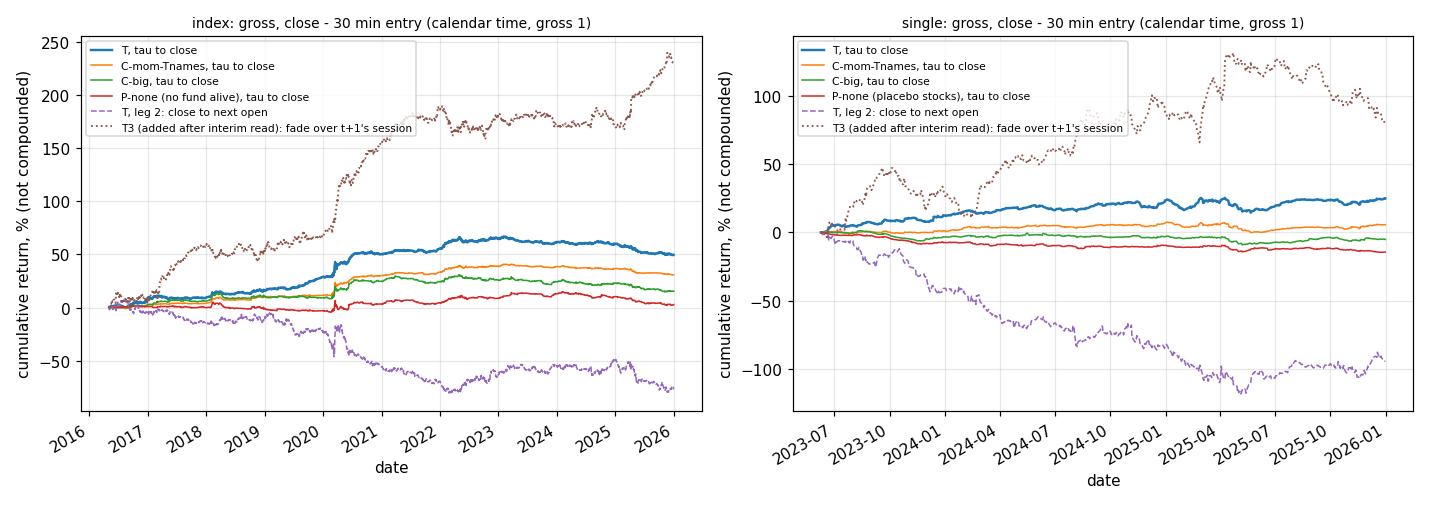
\includegraphics[width=0.8\textwidth]{figures/fig11_etf_equity.png}
\caption{Cumulative gross return, not compounded, entry 30 minutes before the close, reproduced from the study's output (its daily series are not among the published aggregates). Left: index and sector ETFs, 2016--2025. Right: single stocks with leveraged funds, from June 2023. ``T3'' is a next-session fade added after an interim read (Section~\ref{sec:c_leads}).}
\label{fig:c_eq}
\qsource{Alpaca SIP bars, quotes and auction prints; CRSP via WRDS; author's calculations.}
\end{figure*}

Table~\ref{tab:c_index} and Figure~\ref{fig:c_eq} give leg 1. T earned 1.9\,bp an event (Sharpe 0.97, $t$ 3.0) with about four events a day in 28 ETFs, and the placebos with little or no leveraged money earned nothing. But plain momentum on the same ETFs, every day, earned a Sharpe of 0.92. Table~\ref{tab:c_add} asks directly whether the flow's size adds. Regressing T's daily P\&L on C-mom-Tnames leaves an alpha of 0.45\,bp a day with $t$ 1.22; within an ETF, a larger predicted flow does not predict a larger move into the close ($t$ $-$1.22). What separates T from the placebos is which ETFs it holds (semiconductors, biotechnology, gold miners, aerospace: SOXX, XBI and ITA carry 39\% of its events), not when it holds them; without those three ETFs the book is 0.78. The dose response is flat (Figure~\ref{fig:c_dose}): by $S$ as a multiple of $S^{*}$ on big-move days, the per-event return is +2.6, +6.4, +5.4, +4.0 and +5.5\,bp from the lowest bin to the highest. By the flow against the auction's usual size the top fifth earns +6.6\,bp against +2.5\,bp in the bottom fifth, but a book built on that measure scores 0.80, below T.

\begin{table}[H]
\centering
\caption{Does the flow's size add to momentum? Leg 1, index group, 2016--2025. HAC errors (5 lags); pooled regressions clustered by date.}
\label{tab:c_add}
\footnotesize
\qstripes
\begin{tabularx}{\columnwidth}{@{}>{\raggedright\arraybackslash}Xr@{}}
\toprule
\qhead{Test} & \qhead{Result} \\
\midrule
T on C-mom-Tnames: alpha, bp/day ($t$) & 0.45 (1.22) \\
\quad beta; $R^2$ & 1.25; 0.69 \\
T on C-big: alpha ($t$) & 1.54 (3.24) \\
T on C-mom: alpha ($t$) & 0.99 (2.51) \\
Pooled: coefficient on $S$ ($t$) & $-$0.011 ($-$0.83) \\
Within each ETF: coefficient on $S$ ($t$) & $-$0.027 ($-$1.22) \\
\bottomrule
\end{tabularx}
\qsource{Alpaca SIP bars, quotes and auction prints; CRSP via WRDS; author's calculations.}
\end{table}

\begin{figure}[tbp]
\centering
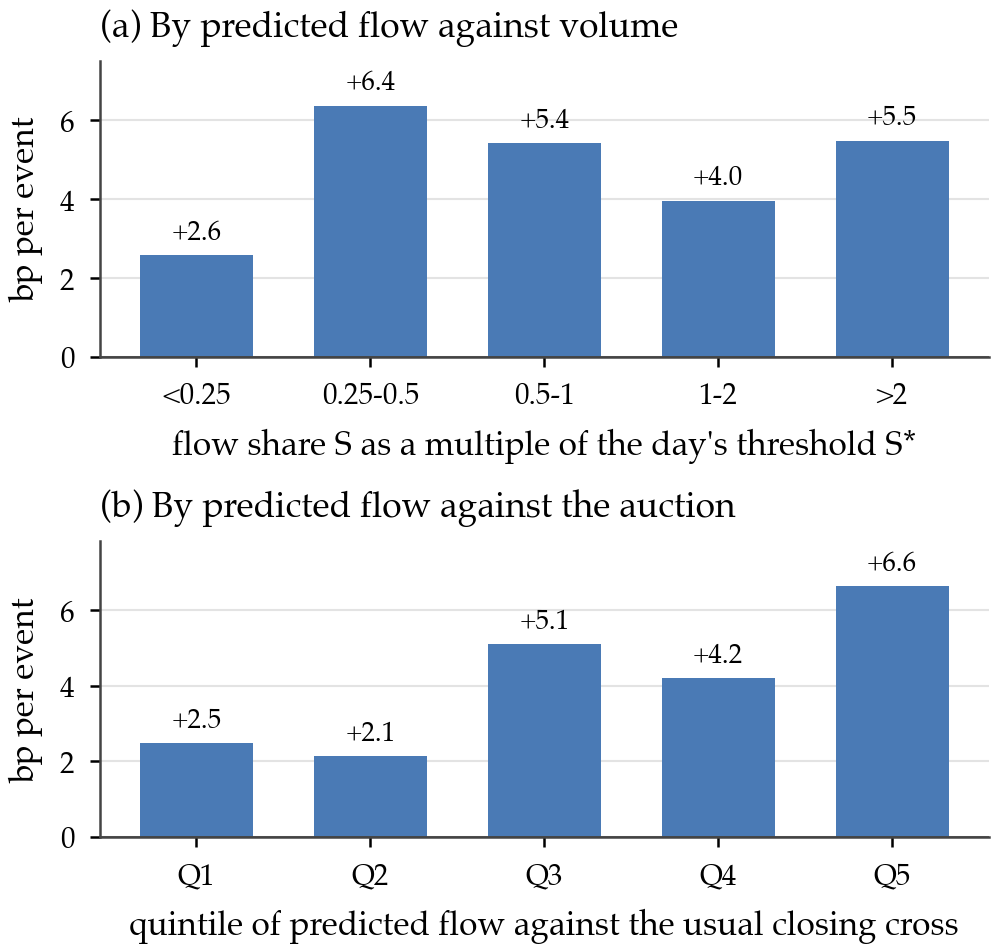
\includegraphics[width=\columnwidth]{figures/fig14_dose.png}
\caption{Dose response, leg 1, big-move days with a leveraged fund alive, index group, 2016--2025: mean gross return per event by the predicted flow against daily volume (a, as a multiple of the day's threshold) and against the ETF's usual closing cross (b, quintiles).}
\label{fig:c_dose}
\qsource{Alpaca SIP bars, quotes and auction prints; CRSP via WRDS; author's calculations.}
\end{figure}

\textbf{Time.} Figures~\ref{fig:c_year} and \ref{fig:c_heat} show the effect decaying. T's Sharpe was 1.67 in 2016--2022 and $-$1.32 in 2023--2025 ($t$ $-$2.3), and the same-name momentum control fell with it. Per event T earned +8.3\,bp in 2020 and $-$4.6\,bp in 2025 ($t$ $-$2.52), against a quoted half-spread that fell from about 1.5 to 0.9\,bp. The edge was largest when leveraged assets were smallest: the index group's funds held \$22bn on average in 2016 and \$91bn in 2025, and $k$ rose from \$118bn to \$487bn, while the effect went from positive to negative. That is the opposite of what the mechanism predicts. In 2026, out of sample on ProShares-only assets (about half of the flow), T scored $-$1.28 ($t$ $-$1.29) on 467 events. Leg 2, from the close to the next open, lost: T $-$0.52 ($t$ $-$1.67), $-$2.7\,bp an event.

\begin{figure}[tbp]
\centering
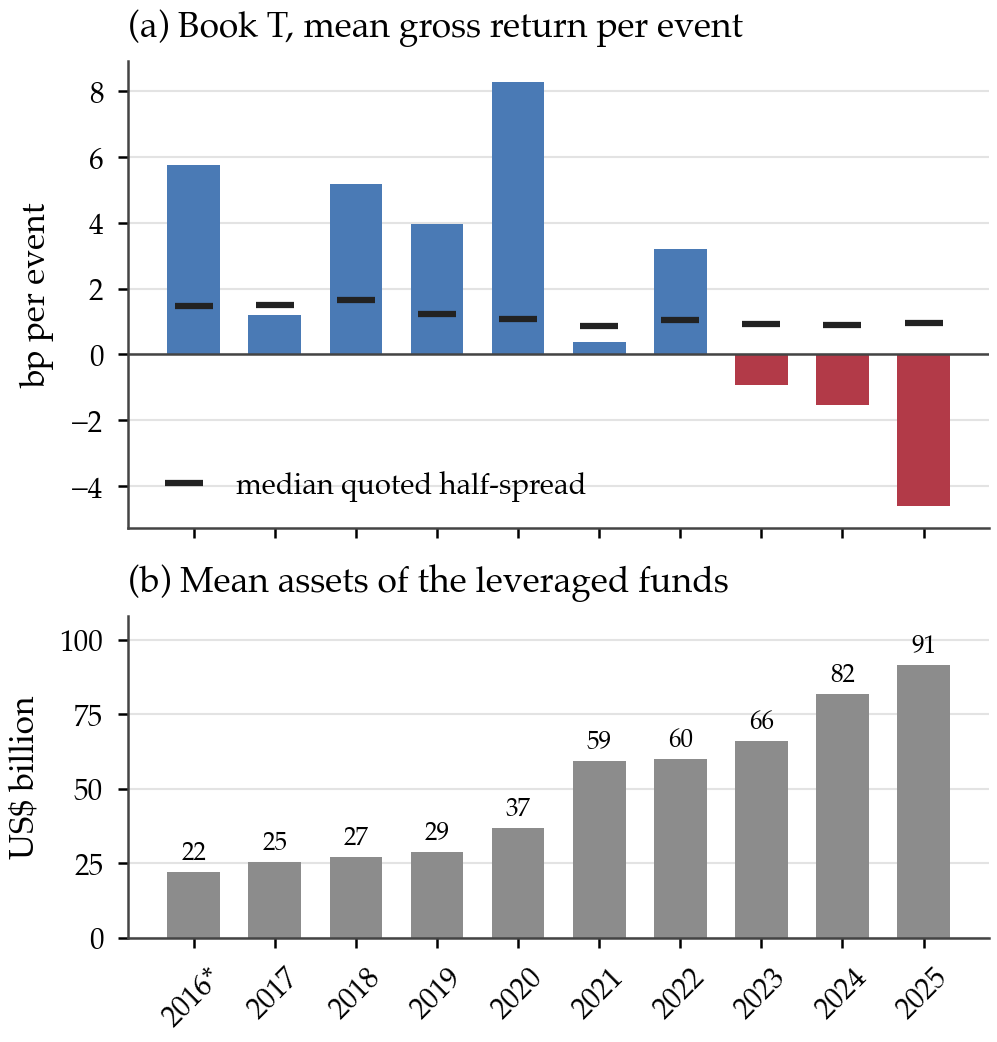
\includegraphics[width=\columnwidth]{figures/fig12_etf_year.png}
\caption{(a) Book T, leg 1: mean gross return per event by year, bp, with the median quoted half-spread at entry. (b) Mean assets of the leveraged funds on the index and sector ETFs, US\$ billion. 2016$^{*}$ starts in May.}
\label{fig:c_year}
\qsource{Alpaca SIP bars, quotes and auction prints; CRSP via WRDS; author's calculations.}
\end{figure}

\begin{figure*}[t]
\centering
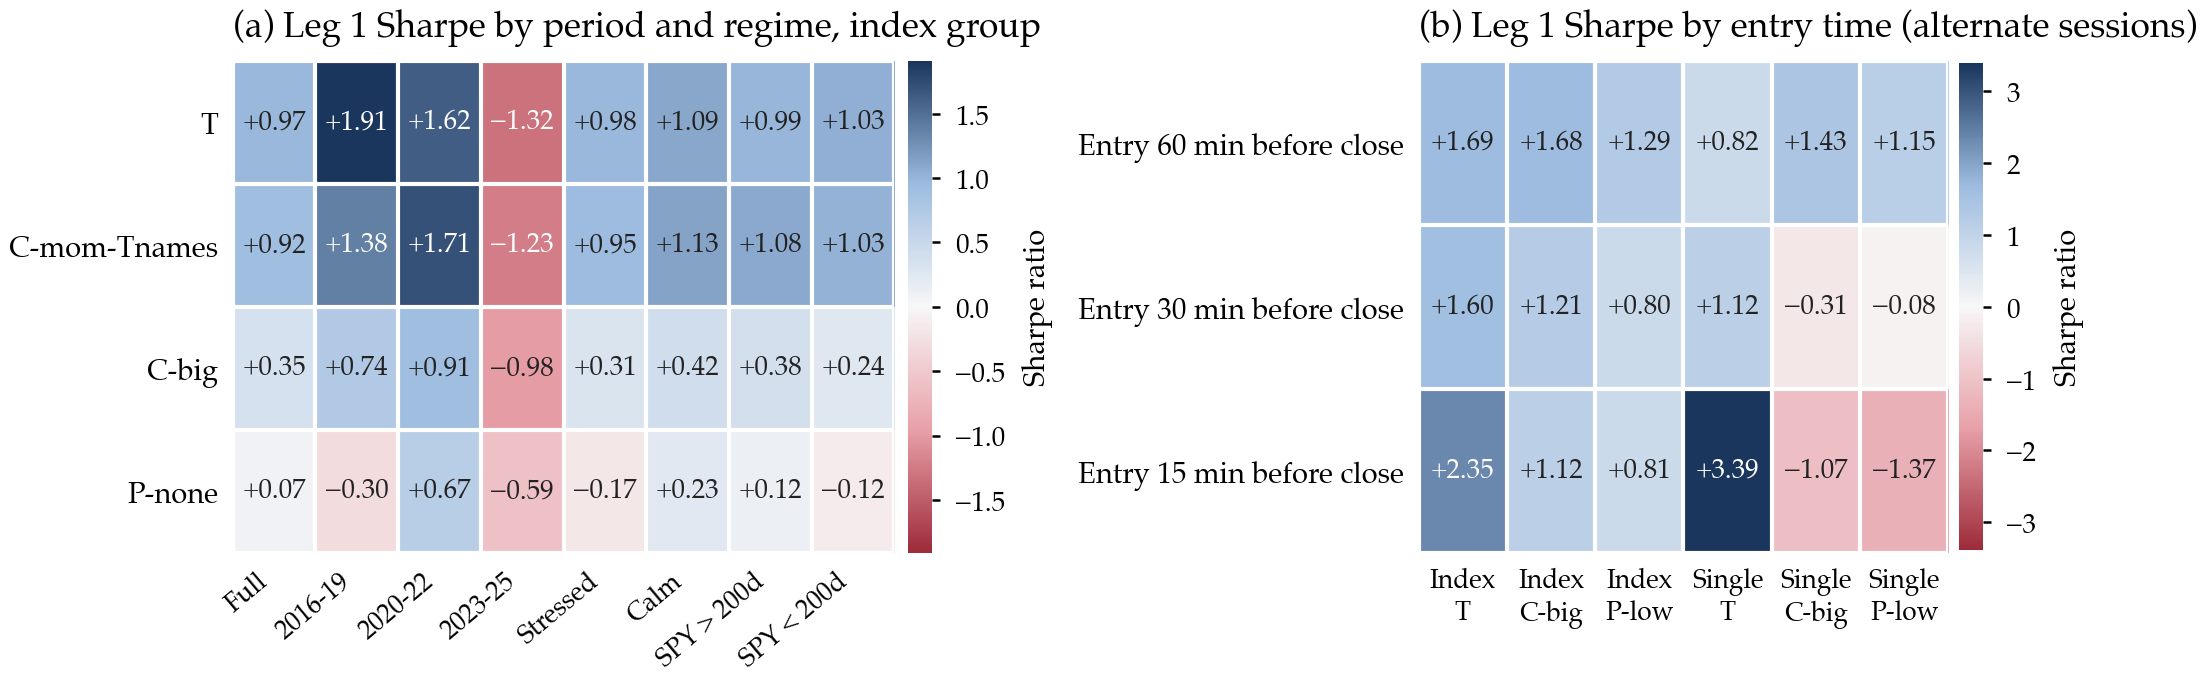
\includegraphics[width=\textwidth]{figures/fig13_etf_heat.png}
\caption{Leg 1 Sharpe ratios, gross. (a) Four books by period and regime, index group, 2016-05-05 to 2025-12-31; stressed means SPY's 21-session volatility of 20\% or more. (b) Entry 60, 30 and 15 minutes before the close, index and single-stock groups, on alternate sessions only (the rows compare with each other, not with panel a).}
\label{fig:c_heat}
\qsource{Alpaca SIP bars, quotes and auction prints; CRSP via WRDS; author's calculations.}
\end{figure*}

\textbf{Neighbouring entry times.} The entries at 60 and 15 minutes before the close were fetched on alternate sessions only, because the market-data request budget was shared with another job on the night of the fetch. On those sessions T is positive at all three entries (Sharpe 1.69, 1.60 and 2.35 with entry 60, 30 and 15 minutes before the close) and so are the big-move controls (1.68, 1.21 and 1.12; Figure~\ref{fig:c_heat}b). With the 15-minute entry T is about twice the control. Every book is better on even-numbered sessions than on odd ones (T 1.57 against 0.45), about two standard errors on books that move together; no fetch pattern explains it, and splits by other session moduli spread as widely, which is consistent with chance.

\subsection{Single stocks}

The point-in-time threshold first exists on 2023-06-09: single-stock leveraged funds were too small before (average assets \$0.12bn in 2022 and \$22bn in 2025). On 3,469 events in 53 stocks to the end of 2025, T scored 1.24 ($t$ 1.69), 3.1\,bp an event against a 1.9\,bp half-spread, and momentum on the same stocks scored 0.51; all-stock momentum and the no-fund placebo lost ($-$1.34 and $-$1.48). Within a stock the size adds nothing ($t$ $-$1.11); TSLA, COIN and NVDA carry 40\% of the events, and without them T is 0.75. Leg 2 lost ($-$1.34, $-$7.6\,bp an event): in these stocks a day's move continues into the next open. On two and a half years and $t$ 1.7, this is a reason to watch the group, not a result.

\subsection{Capacity}

\begin{table}[tbp]
\centering
\caption{Capacity of T, leg 1, 2016--2025: position against ADV and against the ETF's usual closing cross.}
\label{tab:c_cap}
\footnotesize
\setlength{\tabcolsep}{3.2pt}
\qstripes
\begin{tabular}{@{}lrrrrr@{}}
\toprule
\qhead{Book} & \qhead{\makecell[r]{Median\\\% ADV}} & \qhead{\makecell[r]{Max\\\% ADV}} & \qhead{\makecell[r]{Share\\$>$1\% ADV}} & \qhead{\makecell[r]{Median\\\% X}} & \qhead{\makecell[r]{Share\\$>$5\% X}} \\
\midrule
Index \$1M & 0.05 & 4.3 & 2\% & 2.2 & 40\% \\
Index \$5M & 0.24 & 21.4 & 24\% & 11.1 & 63\% \\
Index \$10M & 0.47 & 42.7 & 35\% & 22.2 & 74\% \\
Single \$1M & 0.00 & 0.6 & 0\% & 0.1 & 0\% \\
Single \$10M & 0.04 & 6.0 & 1\% & 0.8 & 13\% \\
\bottomrule
\end{tabular}
\qsource{Alpaca SIP bars and auction prints; CRSP via WRDS; author's calculations.}
\end{table}

The sector ETFs T trades have small closing crosses (``X'' in Table~\ref{tab:c_cap}), because their funds' flow lands in the constituent stocks, so the exit binds rather than the entry: at \$5M most positions exceed 5\% of the ETF's usual cross.

\subsection{Leads found after the rule was fixed}
\label{sec:c_leads}

The study scored about 96 book configurations across eight samples, plus dose bins, per-name and per-year tables. The two leads below are the best of all of that and should be discounted for it.

\textbf{Foreign-market ETFs, leg 2.} On the foreign-market list, where six single-country ETFs carry events (FXI and ASHR carry 78\% of the 749), fading the move from the closing cross to the next opening cross earned a Sharpe of 0.89 ($t$ 3.01), +23.4\,bp an event, positive in each of the ten years. Decomposed, it is a next-session reversal of the home market's move, not of the leveraged funds' trade: on 724 of the 749 events the overnight gap to $t$'s US open has the move's sign, and over every eligible foreign name-day fading the gap earns +3.3\,bp ($t$ 1.88) while fading the US-session part loses $-$1.7\,bp. The subgroup was defined after a development run; the next step, if any, is a separate test of home-market reversal in US-listed single-country ETFs, run forward.

\textbf{Next-session fade (T3).} Deciding after the close on the whole day's move and fading it from $t+1$'s opening cross to its closing cross scored 1.29 ($t$ 3.88; 1.42 in 2016--22 and 0.98 in 2023--25), against 1.14 for plain reversal on the same ETFs (alpha $t$ 2.11). It carries equity beta (SPY 0.186, $t$ 2.4), scored $-$0.84 in 2026 on half the assets, and is mostly a one-day reversal in volatile sector ETFs.

\subsection{Conclusion of the study}

The trade the idea proposed does not work as a leveraged-flow trade. There is momentum into the close in the ETFs that carry large leveraged funds, but plain momentum on the same ETFs does about as well, the flow's size adds nothing within an ETF, and the effect turned negative from 2023 as leveraged assets grew. Per trade it is near the half-spread. The control scores as well as the treatment, so the idea is set aside. It would reopen with the 15-minute entry tested against same-name momentum on every session, with a measure of the funds' net trade after creations and redemptions, or with more years of single-stock data. Its correlation with the CEF book is near zero (leg 1: 0.012 with the core sleeve's backtest, $-$0.046 with the second sleeve's).

%═══════════════════════════════════════════════════════
\section{Robustness and Checks}
\label{sec:robust}

Each study split time at least once and reported at least two regimes named in advance (Figures~\ref{fig:a_fc}, \ref{fig:b_split} and \ref{fig:c_heat}). Each was checked for lookahead by recomputing its signals from data truncated at sample dates (five dates for the beta study, four for the close test, a sample of rows for the forecast); all passed. After the first run each analysis was re-derived from its cached inputs and its code checked against the stated conventions; the defects found were fixed before this paper was written.

\textbf{Auction study.} Nasdaq crosses printed under the second SIP code had been scored as days without a cross; fixing this moved the second sleeve's no-cross share for 2016--2026 from 15.4\% to 12.7\%. Days with no official-close data are now missing, not zero. The live-test size had asked only for an expected $t$ of 2 (31 and 5 sessions); at 80\% power it is 368 and 11. The cap had been sized at 15:45 although the remainder was worked from 14:00; with the pre-open forecast the \$100k MOC share is 57.2\%, not 59.6\%. Cross sizes, the pool and forecast skill did not move.

\textbf{Beta study.} The first placebo re-shuffled betas across funds every day, the wrong control for a persistent quantity; the persistent placebo replaced it. The short-only overlay's controls and the tilt-state uncertainty were added at this stage.

\textbf{Close test.} The flow thresholds had been full-sample quantiles, which read the future; made expanding, T's Sharpe moved from 1.08 to 0.97. Leg-2 and leg-3 returns had been dated a session early; re-dated, the next-session fade's SPY beta moved from $-$0.034 to +0.186. The set-aside conclusion did not change.

%═══════════════════════════════════════════════════════
\section{Limitations}
\label{sec:limits}

\begin{enumerate}[nosep,leftmargin=*]
    \item \textbf{All backtests are gross.} No cost, borrow or slippage model is applied; the auction study measures spreads and trade sizes but estimates no cost.
    \item \textbf{Our auction impact is unmeasured} ($n = 0$). Every participation figure assumes the cross does not move when the book joins it.
    \item \textbf{Paper is not live.} Paper runs no closing auction and charges no borrow; 13 sessions say nothing about return.
    \item \textbf{The 2026 step in cross size is measured, not explained}, and nor is the quarter-end effect.
    \item \textbf{Study 1's policy orders are a model}, and the second sleeve's own orders were not read; Study 2's base has no independent check after 2022.
    \item \textbf{The close test's fund multiples were estimated} rather than read from prospectuses; 2026 uses ProShares' assets only, and fills at the mid are not tested.
\end{enumerate}

%═══════════════════════════════════════════════════════
\section{Conclusion}
\label{sec:conclusion}

The closing auction in these closed-end funds is small, even at its current decade high, and only roughly forecastable 15 minutes before the cut-off. A cap at a fraction of a calibrated low quantile keeps more than half of a \$100k book's notional in the auction, but from \$1M the auction carries a small slice and the afternoon carries the book, and from \$5M the afternoon binds as well. The measurement that matters most, our own impact on the print, needs real money; at the paper book's size about 11 live sessions, scored against the current paper record, would detect a 10\,bp impact. The second sleeve's market tilt is a state it visits rather than a fixed feature. Reweighting the funds to remove it loses about what any comparable constraint loses and adds a large 2009 drawdown, while an index overlay removes the beta at a modest, weakly measured cost and is the candidate for further testing. The leveraged-ETF close trade turned out to be ordinary momentum in the ETFs that happen to carry large leveraged funds, and it has lost money since 2023; it is set aside, with two leads recorded and discounted for the search that found them.

%═══════════════════════════════════════════════════════
\section*{Code Availability}

{\raggedright
The scripts are in this repository under \nolinkurl{code/desk/scripts/cef/close_auction_forecast_2026-11-24/} (Study 1), \nolinkurl{code/desk/scripts/cef/c4_beta_neutral_2026-11-24/} (Study 2) and \nolinkurl{code/desk/results/ideas/levered_etf_close/} (Study 3). They import the desk's public research harness, \texttt{scripts/research/harness.py} in \url{https://github.com/quanttqueensu/CreditTrading}. The data are licensed (CRSP via WRDS) or cached vendor market data (Alpaca, Yahoo Finance, ProShares) and are not distributed; the fetch steps need the user's own market-data access.\par}

%═══════════════════════════════════════════════════════
\begin{thebibliography}{99}
\footnotesize
\setlength{\itemsep}{1pt}

\bibitem{lee1991}
C.~M.~C.\ Lee, A.~Shleifer and R.~H.\ Thaler.
\newblock ``Investor sentiment and the closed-end fund puzzle.''
\newblock \textit{Journal of Finance}, 46(1):75--109, 1991.

\bibitem{pontiff1995}
J.\ Pontiff.
\newblock ``Closed-end fund premia and returns: Implications for financial market equilibrium.''
\newblock \textit{Journal of Financial Economics}, 37(3):341--370, 1995.

\bibitem{pontiff1996}
J.\ Pontiff.
\newblock ``Costly arbitrage: Evidence from closed-end funds.''
\newblock \textit{Quarterly Journal of Economics}, 111(4):1135--1151, 1996.

\bibitem{cherkes2009}
M.\ Cherkes, J.\ Sagi and R.\ Stanton.
\newblock ``A liquidity-based theory of closed-end funds.''
\newblock \textit{Review of Financial Studies}, 22(1):257--297, 2009.

\bibitem{dimson1979}
E.\ Dimson.
\newblock ``Risk measurement when shares are subject to infrequent trading.''
\newblock \textit{Journal of Financial Economics}, 7(2):197--226, 1979.

\bibitem{newey1987}
W.~K.\ Newey and K.~D.\ West.
\newblock ``A simple, positive semi-definite, heteroskedasticity and autocorrelation consistent covariance matrix.''
\newblock \textit{Econometrica}, 55(3):703--708, 1987.

\bibitem{ledoit2008}
O.\ Ledoit and M.\ Wolf.
\newblock ``Robust performance hypothesis testing with the Sharpe ratio.''
\newblock \textit{Journal of Empirical Finance}, 15(5):850--859, 2008.

\bibitem{vasicek1973}
O.~A.\ Vasicek.
\newblock ``A note on using cross-sectional information in Bayesian estimation of security betas.''
\newblock \textit{Journal of Finance}, 28(5):1233--1239, 1973.

\bibitem{cheng2009}
M.\ Cheng and A.\ Madhavan.
\newblock ``The dynamics of leveraged and inverse exchange-traded funds.''
\newblock \textit{Journal of Investment Management}, 7(4):43--62, 2009.

\bibitem{gao2018}
L.\ Gao, Y.\ Han, S.~Z.\ Li and G.\ Zhou.
\newblock ``Market intraday momentum.''
\newblock \textit{Journal of Financial Economics}, 129(2):394--414, 2018.

\bibitem{baltussen2021}
G.\ Baltussen, Z.\ Da, S.\ Lammers and M.\ Martens.
\newblock ``Hedging demand and market intraday momentum.''
\newblock \textit{Journal of Financial Economics}, 142(1):377--403, 2021.

\bibitem{ivanov2018}
I.~T.\ Ivanov and S.~L.\ Lenkey.
\newblock ``Do leveraged ETFs really amplify late-day returns and volatility?''
\newblock \textit{Journal of Financial Markets}, 41:36--56, 2018.

\bibitem{alpacaorders}
Alpaca.
\newblock ``Placing Orders.''
\newblock Documentation, \url{https://docs.alpaca.markets/docs/orders-at-alpaca}, updated October 2026.

\bibitem{alpacapaper}
Alpaca.
\newblock ``Paper Trading.''
\newblock Documentation, \url{https://docs.alpaca.markets/docs/paper-trading}, updated July 2026.

\bibitem{alpacarealtime}
Alpaca.
\newblock ``Real-time Stock Data.''
\newblock Documentation, \url{https://docs.alpaca.markets/docs/real-time-stock-pricing-data}, updated May 2026.

\bibitem{nyseauctions}
New York Stock Exchange.
\newblock ``Auctions'' (auction timetable).
\newblock \url{https://www.nyse.com/trade/auctions}, accessed October 2026.

\bibitem{nyseimbalance}
New York Stock Exchange.
\newblock \textit{Pillar Order Imbalances Feed Client Specification}, version 2.2o, July 30, 2026.

\bibitem{nysepricing}
New York Stock Exchange.
\newblock \textit{Historical Proprietary Market Data Pricing}, as of October 2026.

\bibitem{ctsspec}
Securities Industry Automation Corporation (CTA Plan).
\newblock \textit{CTS Pillar Multicast Output Binary Specification}, version 2.11b, January 29, 2026.

\end{thebibliography}

\end{document}
